\ProvidesPackage{commands}
\documentclass[11pt]{article}
\usepackage{epstopdf}
\usepackage{subfigure,graphicx}
\usepackage{amsmath}
\usepackage{epsf}
\usepackage{amsfonts}
\usepackage{amssymb}
\usepackage{color}
\usepackage{mathtools}
\usepackage{placeins}
\usepackage{booktabs}
\usepackage{enumitem}
\usepackage{caption}
\usepackage[margin=0.8in, paperwidth=8.5in, paperheight=11in]{geometry}
\usepackage{amsfonts}
\usepackage{amsmath}
\usepackage{amsbsy}
\usepackage{authblk}
\usepackage{graphicx}
\usepackage{listings}
\usepackage{array}
\usepackage{titlesec}
\usepackage{amssymb}
\usepackage{bm}
\usepackage{mathtools}
\usepackage{titlesec}

\usepackage[latin1]{inputenc}\newcommand{\bs}[1]{\boldsymbol{#1}}
\newcommand{\del}[2]{\frac{\partial {#1}}{\partial {#2}}}
\newcommand{\D}[2]{\frac{D^{\overline{\alpha}}}{\overline{\alpha !}}{#1}(#2,#2)\ {\bf x}^{\overline{\alpha}}}
\newcommand{\dv}[3]{\frac{{\rm d}^{#1}{#2}}{d{#3}^{#1}}}
\newcommand{\ddel}[5]{\frac{\partial^{ {#1} + {#2}} {#3}}{\partial {#4}^{#1} \partial{#5}^{#2}}}
\newcommand{\dev}{{\rm {\bf dev}}}
\newcommand{\proj}[1]{\frac{1}{R^2}{\bf X}\otimes{\bf X}}
\newcommand{\Ie}[1]{I^{\rm e}_{#1}}
\newcommand{\Ce}[1]{\bf C^{\rm e^{#1}}}
\newcommand{\Fe}[2]{F^{\rm e^{#2}}_{#1}}
\newcommand{\Fv}[2]{F^{\rm v^{#2}}_{#1}}
\newcommand{\f}[2]{f^{\rm {#2}}_{#1}}
\newcommand{\B}[2]{B^{\rm {#2}}_{#1}}
\newcommand{\E}[2]{E^{\rm {#2}}_{#1}}
\newcommand{\fv}[2]{f^{\rm v^{#2}}_{#1}}
\newcommand{\dfv}[2]{\dot{f}^{\rm v^{#2}}_{#1}}
\newcommand{\tGam}[2]{\tilde{\Gamma}^{\rm v^{#2}}_{#1}}
\newcommand{\Gam}[2]{\Gamma^{\rm v^{#2}}_{#1}}
\newcommand{\A}[1]{\mathcal{A}_{#1}}
\newcommand{\F}[2]{F^{\rm #2}_{#1}}
\newcommand{\hpeq}{\hat{\psi}^{\rm Eq}}
\newcommand{\hpneq}{\hat{\psi}^{\rm NEq}}
\newcommand{\etak}{\eta_K({I_1,I_2,J},{\bf C^{\rm e}, B^{\rm v}})}
\newcommand{\nuk}{\nu_K({I_1,I_2,J},{\bf C^{\rm e}, B^{\rm v}})}
\newcommand{\thetak}{\theta_K({I_1,I_2,J},{\bf C^{\rm e}, B^{\rm v}})}
\newcommand{\etaj}{\eta_J({I_1,I_2,J},{\bf C^{\rm e}, B^{\rm v}})}
\newcommand{\dFv}[2]{\dot{F}^{\rm v^{#2}}_{#1}}
\newcommand{\hatpsi}{\widehat{\psi}(I_1, I_2,I^{\rm e}_1,I^{\rm e}_2,J)}
\newcommand{\hpsi}{\widehat{\psi}(I_1,I^{\rm e}_1,J)}
\newcommand{\Fh}[1]{\widehat{\mathcal{F}}\left({\bf F, \Fv{}{}}, {#1}\right)}
\newcommand{\Fhstar}[1]{\widehat{\mathcal{F}}^*\left({\bf F, \Fv{}{}}, {#1}\right)}
\newcommand{\sbar}{\overline{\bm{\sigma}}}
\newcommand{\hpsicomp}[1]{\sum_{r=1}^{2}\left\{\frac{3^{1-\alpha_r}}{2\alpha_r}\mu_r(I^{\alpha_r}_1-3^{\alpha_r})
+\frac{3^{1-a_r}}{2a_r}m_r({\Ie{1}}^{^{a_r}}-3^{a_r})\right\}
+\mu{#1}+\kappa{#1}^2}
\newcommand{\Ni}[1]{N^{(e)}_i(#1)}
\newcommand{\hNi}[1]{\hat{{N}}^{(e)}_i(#1)}
\newcommand{\Ld}{L^{\dagger}}
\newcommand{\intinfinf}{\int_{-\infty}^{\infty} \int_{-\infty}^{\infty}}
\newcommand{\LLnorm}[1]{\left\lVert{#1}\right\rVert_2}
\newcommand{\Linorm}[1]{{\left\lVert{#1}\right\rVert_\infty}}
\newcommand{\tr}{\rm tr}
\newcommand{\deldel}[2]{\frac{\partial^2 {#1}}{\partial {#2}^2}}
\newcommand{\kd}[1]{\delta_{#1}}
\newcommand{\Fie}[1]{{\bf F}^{#1}}
\newcommand{\Comp}{\emph{CompStrainStress\_Cee570.m}}
\newcommand{\Comps}{\emph{CompStrainStress\_Elem\_Cee570.m}}
\newcommand{\Feap}{\emph{FEA\_Program.m}}
\newcommand{\Elast}{\emph{Elast2d\_Elem.m}}
\newcommand{\Assem}{\em{AssemStifForc.m}}
\newcommand{\Fb}{\em{F\_bar\_int}}
\newcommand{\Form}{\em{FormFE.m}}
\newcommand{\Sol}{\em{SolveFE.m}}
\newcommand{\inpt}{\em{triangtwo.m}}

\titlespacing\section{10pt}{10pt plus 4pt minus 2pt}{10pt plus 2pt minus 2pt}
\titlespacing\subsection{0pt}{8pt plus 4pt minus 2pt}{8pt plus 2pt minus 2pt}
\titlespacing\subsubsection{0pt}{12pt plus 4pt minus 2pt}{6pt plus 2pt minus 2pt}
\titlespacing*{\title}{-2ex}{*-2ex}{-2ex}
\usepackage{color} %red, green, blue, yellow, cyan, magenta, black, white
\definecolor{mygreen}{RGB}{28,172,0} % color values Red, Green, Blue
\definecolor{mylilas}{RGB}{170,55,241}
\setlength\parindent{0pt}
\graphicspath{{Figures/}}

\title{\bf CEE 576: Nonlinear Finite Elements \\ Midterm Exam}
\author{Bhavesh Shrimali \\ NetID: bshrima2}
\date{\today}
\begin{document}
\maketitle \hrule \hrule \hrule
\section*{Sol$^n$ 1: }
Given strain energy density function: 
\[
W({\bm\varepsilon}) = a\varepsilon_{ii} \ln(1+\varepsilon_{jj}) + \frac{3}{2} b\varepsilon_{ij}\varepsilon_{ij}
\]\hrule
\subsection*{(a): Stress Tensor and Tensor of Material Modulii}
The Cauchy-stress tensor and the tensor of material modulii can be given by: 
\begin{align*}
\sigma_{ij}
& =\del{W}{\varepsilon_{ij}} = 
a\ln(1+\varepsilon_{rr})\delta_{ij} + a\frac{\varepsilon_{rr}}{1+\varepsilon_{ll}}\delta_{ij}
+ \frac{3}{2}\ 
b\ 
2\varepsilon_{ij}\\
\sigma_{ij}
& = 
a\left( 
\ln (1+\varepsilon_{rr}) + \frac{\varepsilon_{rr}}{1+\varepsilon_{rr}}
\right)\delta_{ij}
+3b\varepsilon_{ij}\\
c_{ijkl}
& = \frac{\partial^2 W}{\partial\varepsilon_{ij}\partial\varepsilon_{kl}} =
\frac{a}{1+\varepsilon_{rr}}\delta_{ij}\delta_{kl}
+\frac{a}{(1+\varepsilon_{rr})^2}\delta_{ij}\delta_{kl}
+\frac{3}{2}b(\delta_{ik}\delta_{jl}+\delta_{il}\delta_{jk})\\
c_{ijkl}
& = 
a\left(
\frac{2+\varepsilon_{rr}}{(1+\varepsilon_{pp})^2}
\right)\delta_{ij}\delta_{kl}
+\frac{3}{2}b(\delta_{ik}\delta_{jl}+\delta_{il}\delta_{jk})
\end{align*}
Hence the Cauchy Stress tensor is given by
\[
\boxed{\sigma_{_{ij}} = a\left( \ln(1+\varepsilon_{rr})\delta_{ij} + \frac{\varepsilon_{rr}}{1+\varepsilon_{ll}}\delta_{ij}\right)
+ 3\ 
b\ 
\varepsilon_{ij}}
\]
and the tensor of material modulii is given by
\[
\boxed{c_{_{ijkl}}=a\left(
\frac{2+\varepsilon_{rr}}{(1+\varepsilon_{pp})^2}
\right)\delta_{ij}\delta_{kl}
+\frac{3}{2}b(\delta_{ik}\delta_{jl}+\delta_{il}\delta_{jk})}
\]
\subsection*{(b): Major and Minor Symmetries of $c_{ijkl}$}
The major and minor symmetries of the tensor of material modulii are verified below. Note that we make use of the symmetric nature of the infinitesimal stress tensor $\bm\varepsilon$, i.e. $\varepsilon_{ij} = \varepsilon_{ji}$
\begin{align}
c_{ijkl}
& = 
a\left(
\frac{2+\varepsilon_{rr}}{(1+\varepsilon_{rr})^2}
\right)\delta_{ij}\delta_{kl}
+\frac{3}{2}b(\delta_{ik}\delta_{jl}+\delta_{il}\delta_{jk})\\
\nonumber c_{klij}
& = 
a\left(
\frac{2+\varepsilon_{rr}}{(1+\varepsilon_{rr})^2}
\right)\delta_{kl}\delta_{ij}
+\frac{3}{2}b(\delta_{ki}\delta_{lj}+\delta_{kj}\delta_{li})\\
& =
a\left(
\frac{2+\varepsilon_{rr}}{(1+\varepsilon_{rr})^2}
\right)\delta_{kl}\delta_{ij}
+\frac{3}{2}b(\delta_{ik}\delta_{jl}+\delta_{jk}\delta_{il})\\
\nonumber c_{jikl}
& = 
a\left(
\frac{2+\varepsilon_{rr}}{(1+\varepsilon_{rr})^2}
\right)\delta_{ji}\delta_{kl}
+\frac{3}{2}b(\delta_{jk}\delta_{il}+\delta_{jl}\delta_{ik})\\
\nonumber & = 
a\left(
\frac{2+\varepsilon_{rr}}{(1+\varepsilon_{rr})^2}
\right)\delta_{ij}\delta_{kl}
+\frac{3}{2}b(\delta_{jk}\delta_{il}+\delta_{jl}\delta_{ik})\\
\nonumber c_{ijlk}& = 
a\left(
\frac{2+\varepsilon_{rr}}{(1+\varepsilon_{rr})^2}
\right)\delta_{ij}\delta_{lk}
+\frac{3}{2}b(\delta_{il}\delta_{jk}+\delta_{ik}\delta_{jl})\\
& = 
a\left(
\frac{2+\varepsilon_{rr}}{(1+\varepsilon_{rr})^2}
\right)\delta_{ij}\delta_{kl}
+\frac{3}{2}b(\delta_{il}\delta_{jk}+\delta_{ik}\delta_{jl})
\end{align}
From the equivalence of (1), (2), (3) and (4) it is plain that the tensor of material modulii has major and minor symmetries. \\ \hrule
\subsection*{(c): }
Using the constitutive relation for elastic materials
\[
\sigma_{ij} = 
c_{_{ijkl}}({\bm\varepsilon})\varepsilon_{_{kl}}\ ; \ \ \ c_{_{ijkl}} = a\left(
\frac{2+\varepsilon_{rr}}{(1+\varepsilon_{pp})^2}
\right)\delta_{ij}\delta_{kl}
+\frac{3}{2}b(\delta_{ik}\delta_{jl}+\delta_{il}\delta_{jk}) 
\]
where $c_{_{ijkl}}$ has major and minor symmetries as noted above, we have 
\begin{align*}
\begin{Bmatrix}
\sigma_{11} \\ \sigma_{22} \\ \sigma_{12}
\end{Bmatrix}
=
\begin{bmatrix}
c_{_{1111}} & c_{_{1122}} & c_{_{1112}} \\
c_{_{2211}} & c_{_{2222}} & c_{_{2212}}\\
c_{_{1211}} & c_{_{1222}} & c_{_{1212}} 
\end{bmatrix}
\begin{bmatrix}
\varepsilon_{_{11}} \\ \varepsilon_{_{22}} \\ 2\varepsilon_{_{12}}
\end{bmatrix}
\end{align*}
We use the following notation 
\[
\tr{\bm\varepsilon} = \varepsilon_{rr} \implies \tr{\bm\varepsilon} = \varepsilon_{_{11}}+\varepsilon_{_{22}}
\]
Substituting the values of $c_{_{ijkl}}$ from above, we get
\begin{align*}
c_{_{1111}} & = 
a\left(
\frac{2+\tr{\bm\varepsilon}}{(1+\tr{\bm\varepsilon})^2} \right)+
3b \\
c_{_{1122}} & = 
a\left(
\frac{2+\tr{\bm\varepsilon}}{(1+\tr{\bm\varepsilon})^2} \right) \\
c_{_{1112}} & = 
0\\
c_{_{2222}}
& = 
a\left(
\frac{2+\tr{\bm\varepsilon}}{(1+\tr{\bm\varepsilon})^2} \right)+
3b\\
c_{_{2212}}
& = 
0\\
c_{_{1212}}& = 
\frac{3}{2}b 
\end{align*}
Thus the $\bf D$ matrix for 2-D plane-strain elasticity associated with the above $c_{_{ijkl}}$ is as follows (Let $\kappa = \frac{2+\tr{\bm\varepsilon}}{(1+\tr{\bm\varepsilon})^2}$), then: 
\[
{\bf D}(\bm\varepsilon)
=
\begin{bmatrix}
a\kappa +
3b
& a\kappa 
& 0 \\
a\kappa 
& a\kappa+
3b
& 0 \\
0
& 0
& 
\frac{3}{2}b
\end{bmatrix}
\]\hrule
\section*{Sol$^n$ 2: }
Considering small strain nonlinear elastic material given in Q-1
\begin{align*}
{\rm div} {\bm\sigma}+{\bf f} 
& ={\bf 0}\ ; \ \ \ \ \sigma_{_{ij}} = a\left( 
\ln (1+\varepsilon_{rr}) + \frac{\varepsilon_{rr}}{1+\varepsilon_{pp}}
\right)\delta_{ij}
+3b\varepsilon_{ij}\\
& \implies \del{\sigma_{_{ij}}}{x_j}+f_i = 0 \implies \del{\sigma_{_{ij}}}{\varepsilon_{_{pq}}}\del{\varepsilon_{_{pq}}}{x_j}+f_i = 0 \implies \del{\varepsilon_{_{pq}}}{x_j}c_{_{ijpq}} + f_i = 0
\end{align*}
\subsection*{(a): Strong Form}
The strong form of the balance of linear momentum, for a general problem, is given by the system of equations: 
\begin{align*}
\left( a\left(
\frac{2+\varepsilon_{rr}}{(1+\varepsilon_{ll})^2}
\right)\delta_{ij}\delta_{pq}
+\frac{3}{2}b(\delta_{ip}\delta_{jq}+\delta_{iq}\delta_{jp})\right)
\del{\varepsilon_{_{pq}}}{x_j}+f_i = 0 \\ 
a\left(
\frac{2+\varepsilon_{rr}}{(1+\varepsilon_{_{ll}})^2}
\right)\del{\varepsilon_{_{pp}}}{x_i}
+ 
3b\del{\varepsilon_{_{ij}}}{x_j} + f_i = 0
\end{align*}
For the special-case of 2-D small strain nonlinear elasticity, we have
\begin{align}
\sigma_{_{11,1}} + \sigma_{_{12,2}} + f_1 = 0\ ; \ \ \ \ 
\sigma_{_{12,1}} + \sigma_{_{22,2}} + f_2 = 0
\label{Strong Form}
\end{align}
For the present problem, we do not consider the body forces ($\bf f = 0$), and hence, the strong form of the governing equations can be expressed as
\begin{align*}
\boxed{{\rm div}{\bm\sigma}({\bm\varepsilon}) = {\bf 0}\ ; \ \ \ \ \ \text{where}\ \ \  {\bm\sigma} = \del{W}{\bm\varepsilon}({\bm\varepsilon})}
\end{align*}
or in indicial form
\begin{align*}
\boxed{a\left(
\frac{2+\varepsilon_{rr}}{(1+\varepsilon_{_{ll}})^2}
\right)\del{\varepsilon_{_{pp}}}{x_i}
+ 
3b\del{\varepsilon_{_{ij}}}{x_j} = 0}
\end{align*}\hrule
\subsection*{(b): Weak form }
We proceed by multiplying the strong form, given by equation (\ref{Strong Form}), with a test function, $w(x,y)$, to develop the weak form for 2-D small strain nonlinear elasticity. 
\subsubsection*{(i): }
The arguments of the functions are ignored for the sake of brevity. More generally 
\begin{align*}
& \int_{\Omega} w_i\sigma_{ij,j}({\bm\varepsilon})\ d\Omega = 0\\
\implies & \int_{\Omega} ((w_i\sigma_{ij}),_{j} - w_{i,j}\sigma_{ij})\ d\Omega = 0\\
\implies & \int_{\Gamma_h} w_i\sigma_{ij}n_j\ d\Gamma = \int_{\Omega} w_{i,j}\sigma_{ij}(\varepsilon)\ d\Omega\\
\implies & \int_{\Gamma_h} w_ih_i\ d\Gamma = \int_{\Omega} w_{i,j}\sigma_{ij}(\varepsilon)\ d\Omega
\end{align*}
Thus the weak form of the governing equations can be given by
\begin{align}
\boxed{\int_{\Gamma_h} w_ih_i\ d\Gamma = \int_{\Omega} w_{i,j}\sigma_{ij}(\varepsilon)\ d\Omega\ \ \ \ \forall w_i \in {\bf H}^1(\Omega)\ \ ;\ \Omega = \left\{ 0 < x,y < 1\right\}\ 
\ ; \ \ 1 \leq i,j \leq 2}
\end{align}
And the boundaries are given by
\begin{align*}
\boxed{{\bf\text{For Problem 3 and 4 }}\ ;\ \ \Gamma_{_g} = \left\{ x\ |\ x = 0\right\}\ ; \ \Gamma_{_h} = \left\{ x \ |\  x = 1\right\}}
\end{align*}
\subsubsection*{(ii): }
Given below are the functional spaces for the test function, $w(x,y)$, that are relevant for description of the weak form. (Note: ${\bf H}^1(\Omega)$ refers to the Sobolev Space of functions over the domain $(\Omega)$. {$L^2(\Omega)$} refers to the space of square integrable (Lebesgue) functions over the domain $(\Omega)$) 
\begin{align*}
{\bf H}^1({\Omega}) & = \begin{Bmatrix}
w(x,y) &; & w(x,y) \in L^2(\Omega), & {w_x,w_y}\in L^2(\Omega) 
\end{Bmatrix}\\
L^2({\Omega}) & = 
\begin{Bmatrix}
w(x,y) &; & \int_{\Omega} |w(x,y)|^2\ d\Omega\  < \infty
\end{Bmatrix}
\end{align*}
where 
$$w_x = \del{w}{x}(x,y)\ ; w_y = \del{w}{y}(x,y)$$
For the present problem, we require the trial field and the test function to satisfy the following conditions. 
\begin{align*}
u(x,y) \in \mathcal{S}\\
w(x,y) \in \mathcal{V}
\end{align*}
and 
\begin{align*}
\mathcal{S} & = \left\{ u(x,y) \ \|\ \ u\in {\bf H}^1(\Omega)\ \ u|_{_{\Gamma_g}} = u_{_0}  \right\}\\
\mathcal{V} & = \left\{ w(x,y) \ \|\ \ w\in {\bf H}^1(\Omega)\ \ w|_{_{\Gamma_g}} = 0  \right\}\\
\end{align*}
In the above formulation the stress ($\bm\sigma$) is a nonlinear function of strain ($\bm\varepsilon$), which again is a function of the displacement field ($\bm$).
\subsection*{(c): }
The following four node quadrilateral element is used in the analysis. 
\begin{center}
\hspace{-1.5in}
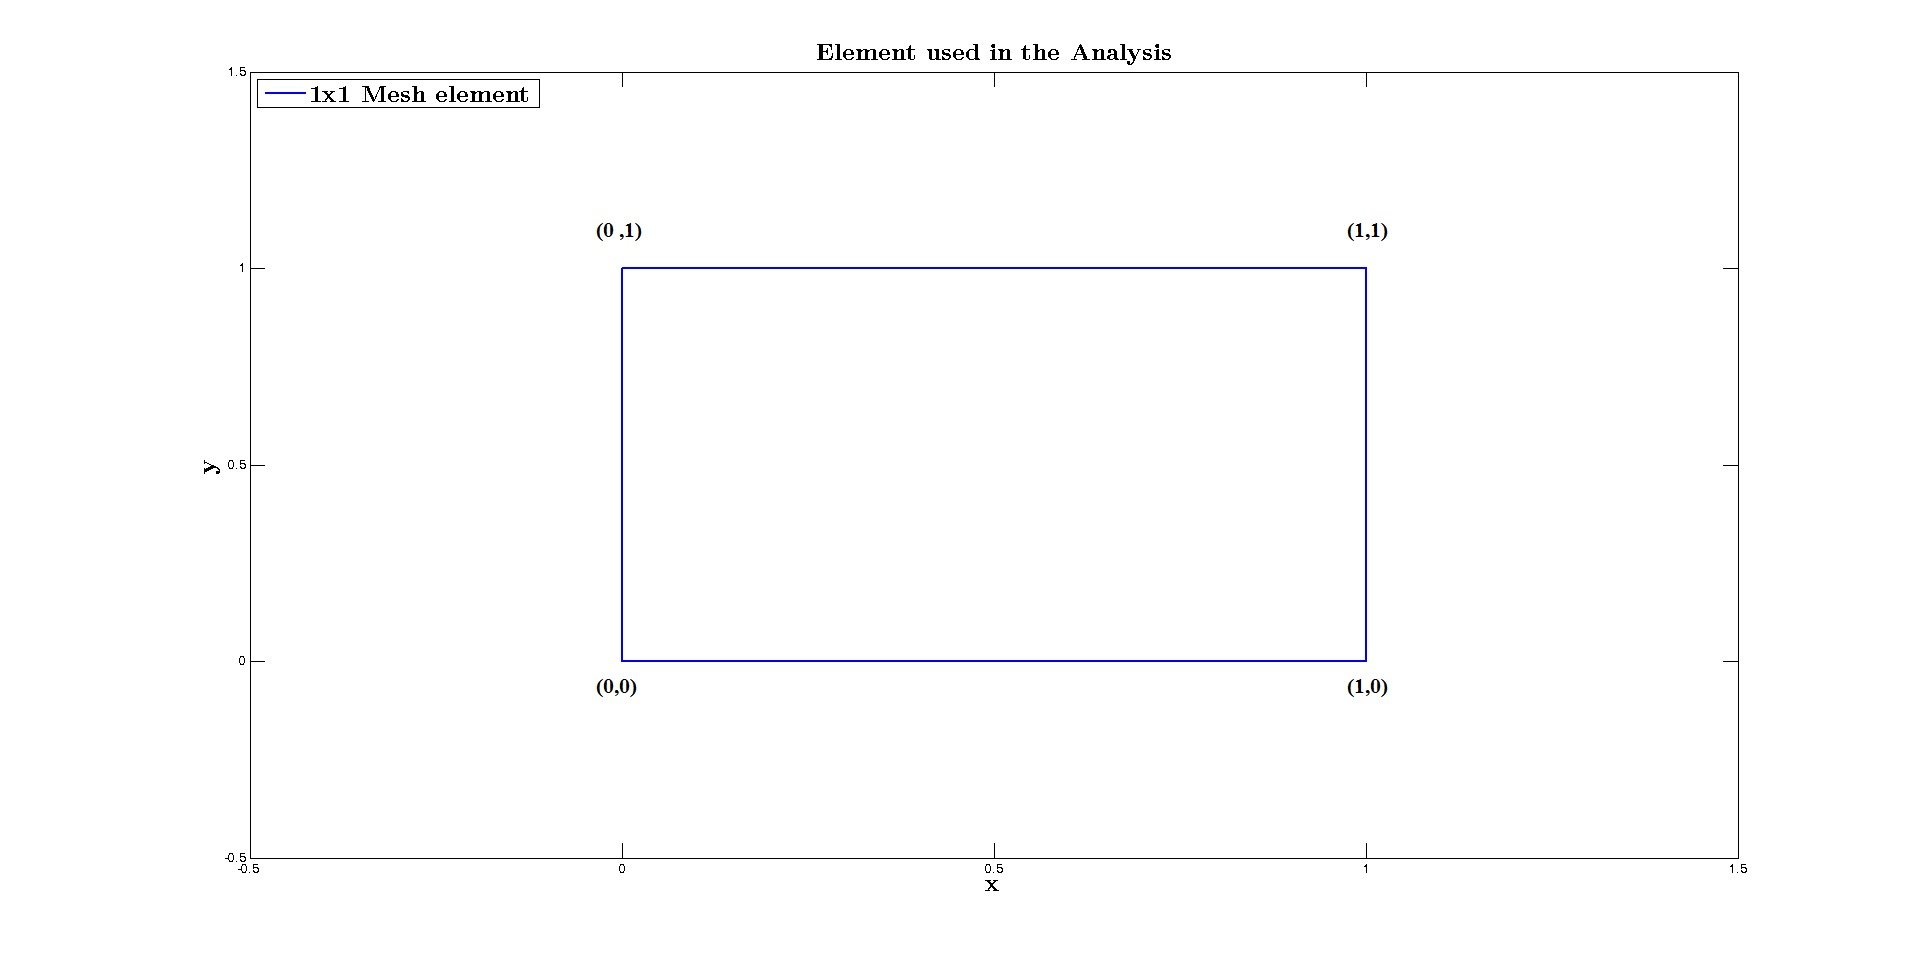
\includegraphics[width=7.in]{Elemente} \\
\end{center}
The canonical domain is as depicted below
\begin{center}
\hspace{-1.5in}
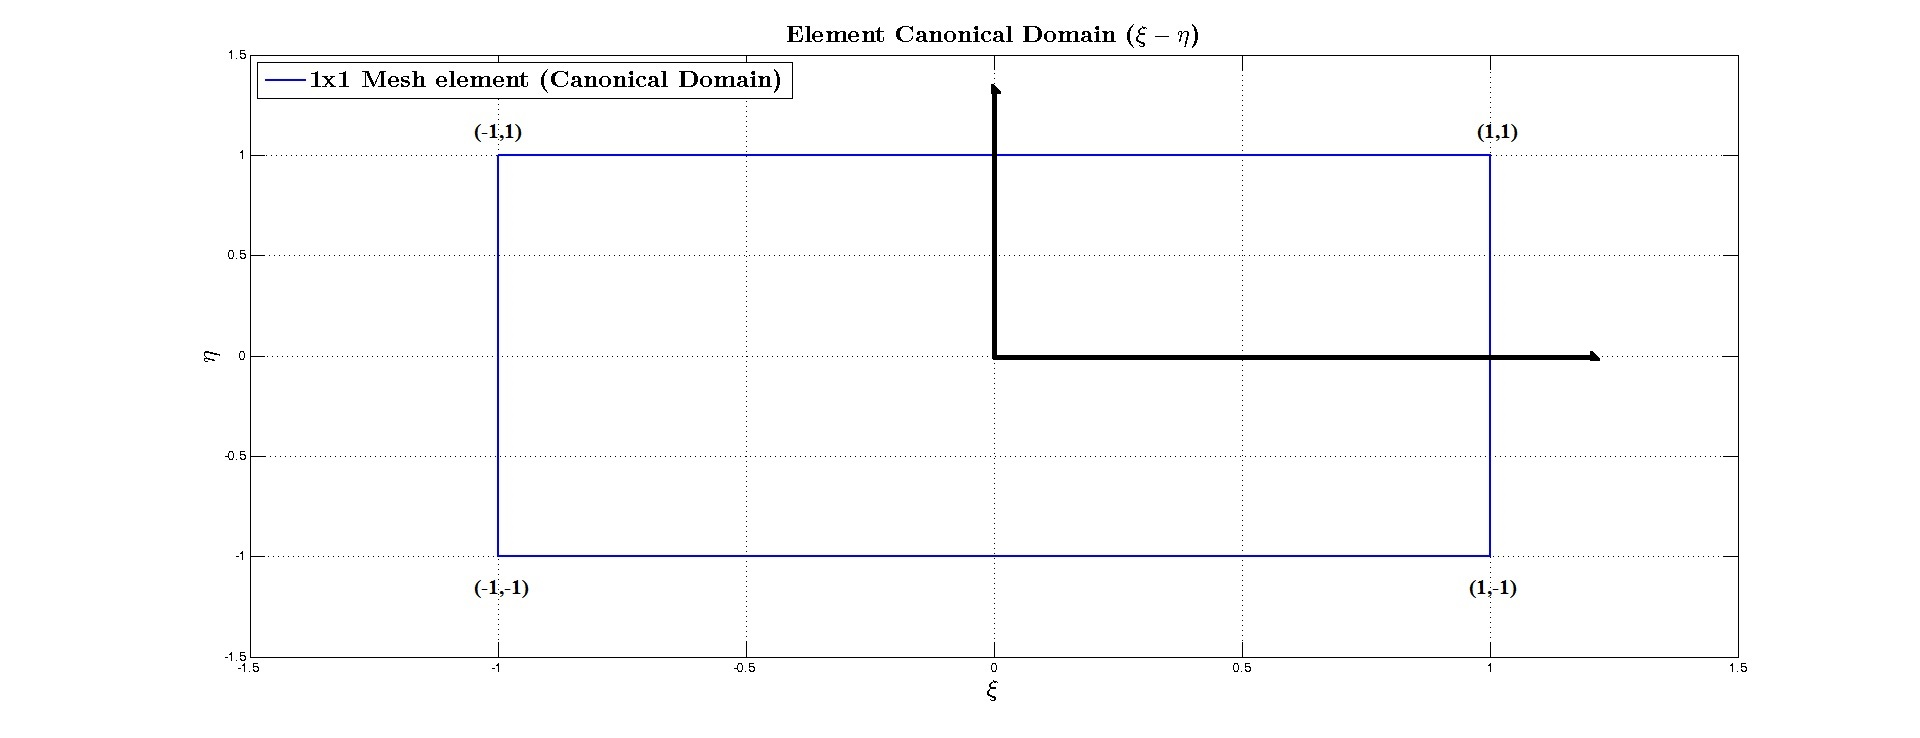
\includegraphics[width=7.5in]{Elementc} \\
\end{center}
The corresponding Lagrange shape functions are
\begin{align*}
\begin{Bmatrix}
N_1(\xi,\eta)\\
N_2(\xi,\eta)\\
N_3(\xi,\eta)\\
N_4(\xi,\eta)
\end{Bmatrix}
=
\frac{1}{4}
\begin{Bmatrix}
(1-\xi) (1-\eta)\\
(1+\xi) (1-\eta)\\
(1+\xi) (1+\eta)\\
(1-\xi) (1+\eta)\\
\end{Bmatrix}
\end{align*}
where $N_i(\xi,\eta)$ denotes the shape function for the $i-th$ node.  \\ \hrule
\subsection*{(e): }
The small-strain non-linear elasticity code is described as follows. 
\begin{itemize}
\item The consistent tangent (stiffness) matrix, ($\bf D(\bm\varepsilon)$), needs to be updated in order to account for the dependence on the strain ($\bm\varepsilon$), leading to the non-linearity. 
\item The Stiffness matrix ($\bf D(\bm\varepsilon)$) needs to be updated in the following subroutines (in order)-
\begin{itemize}
\item \emph{CompStrainStress\_Elem\_Cee570.m}: Lines 125 - 142. 
\item {\Elast} : Line 139 - 159 
\end{itemize} 
\item The subroutine {\Elast} needs an update to generate the element internal force {\em{fint}} which, further needs to be assembled. (Line 157). The assembled internal force ({\Fb}) is first initialized to zero in {\Form} (Line 16).
\item The element internal force vector ({\Fb}) is assembled , from the element internal force, in the assembling subroutine {\Assem} (Line 18)
\item The linearized system is solved for the unknown degrees of freedom, using the residual computed for each load step. The Residual is computed in the subroutine {\Sol} (Line 28-30).
\item This completes one iteration of the Newton Raphson Subroutine, which is built in the input file {\inpt} (Line 175-205)
\end{itemize} \hrule
\section*{Sol$^n$ 3:}
Given material parameters: 
\begin{itemize}
\item a = 40
\item b = 60
\end{itemize}
The following mesh shows the boundary conditions. Some important remarks regarding the mesh are as follows:
\begin{itemize}
\item The bottom left node is constrained both in the x and y directions
\item The top left node is constrained in the x direction
\item During the subsequent mesh refinements, all the nodes on the left edge of the mesh are constrained in the x direction, except the bottom left node which is constrained in both x and y direction
\item Nodal forces $\bf P$ are applied at the right edge along the top and bottom nodes which produce the desired uniaxial strain. 
\item During the subsequent mesh refinements, the nodal forces at the internal nodes on the right edge are double those at the ends. 
\item For compression the entire formulation remains the same, except for the nodal forces, which get reversed in direction. 
\end{itemize}
\begin{center}
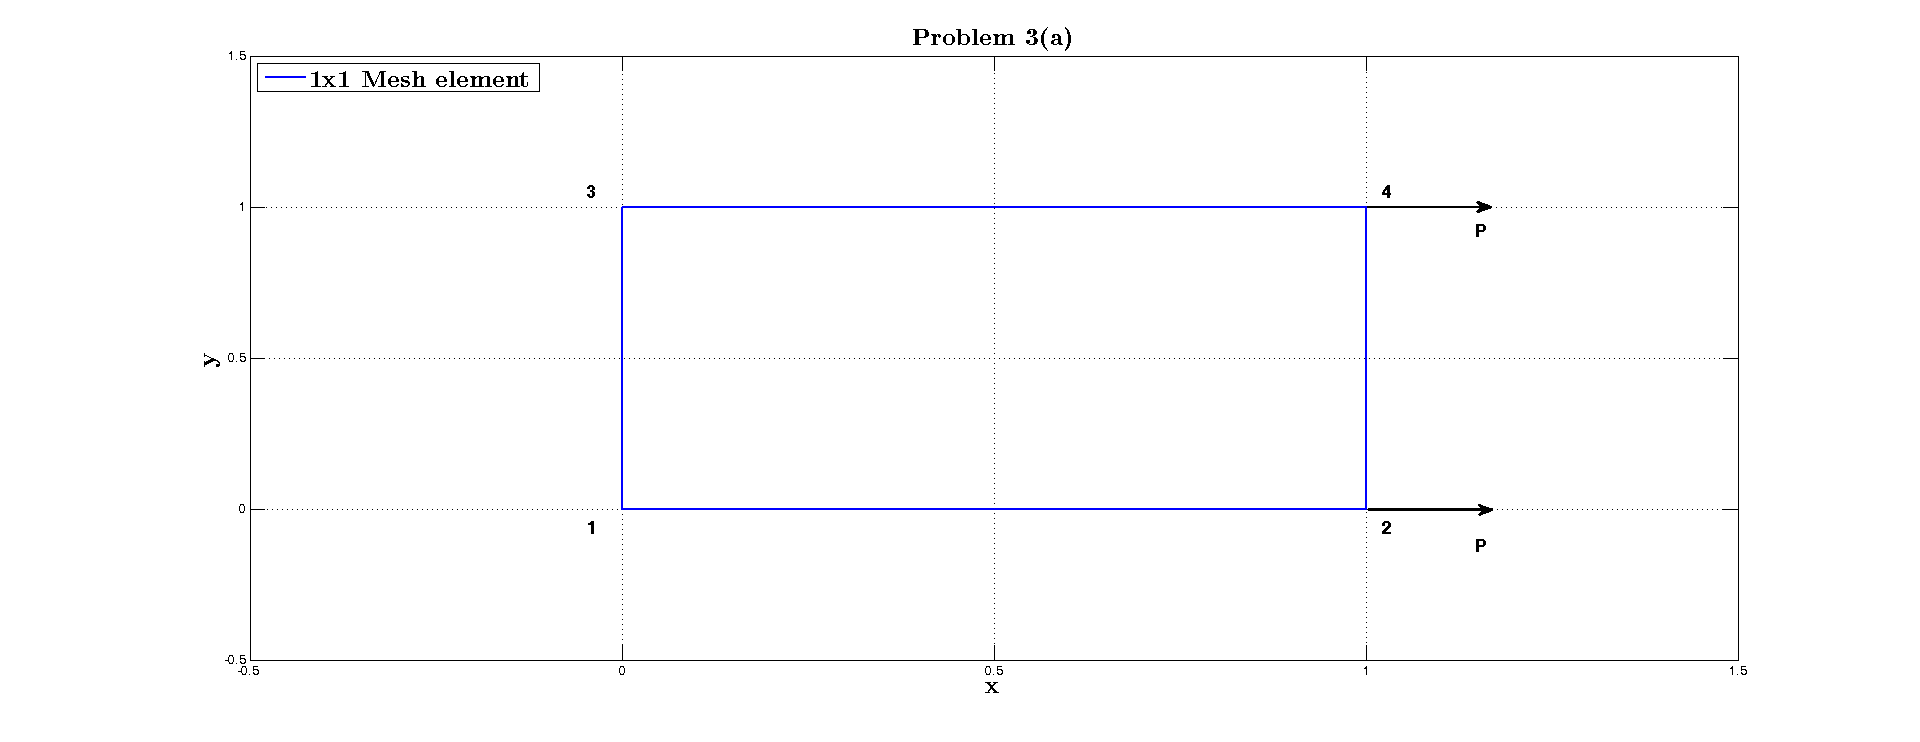
\includegraphics[width=7.0in]{fig3a}
\end{center}
\subsection*{(a): Axial Tension}
The nodal displacements obtained are as follows
\begin{table}[htbp]
  \centering
  \caption{Nodal Displacements for 1x1 mesh (Tension)}
    \begin{tabular}{ccc}
    \toprule
    Node No & $\Delta_x$ & $\Delta_y$ \\
    \midrule
    1     & 0     & 0 \\
    2     & 0.050038 & 0 \\
    3     & 0     & -0.01485 \\
    4     & 0.050038 & -0.01485 \\
    \bottomrule
    \end{tabular}%
  \label{Displacements}%
\end{table}
\begin{itemize}
\item Deformed Shape:
\begin{center}
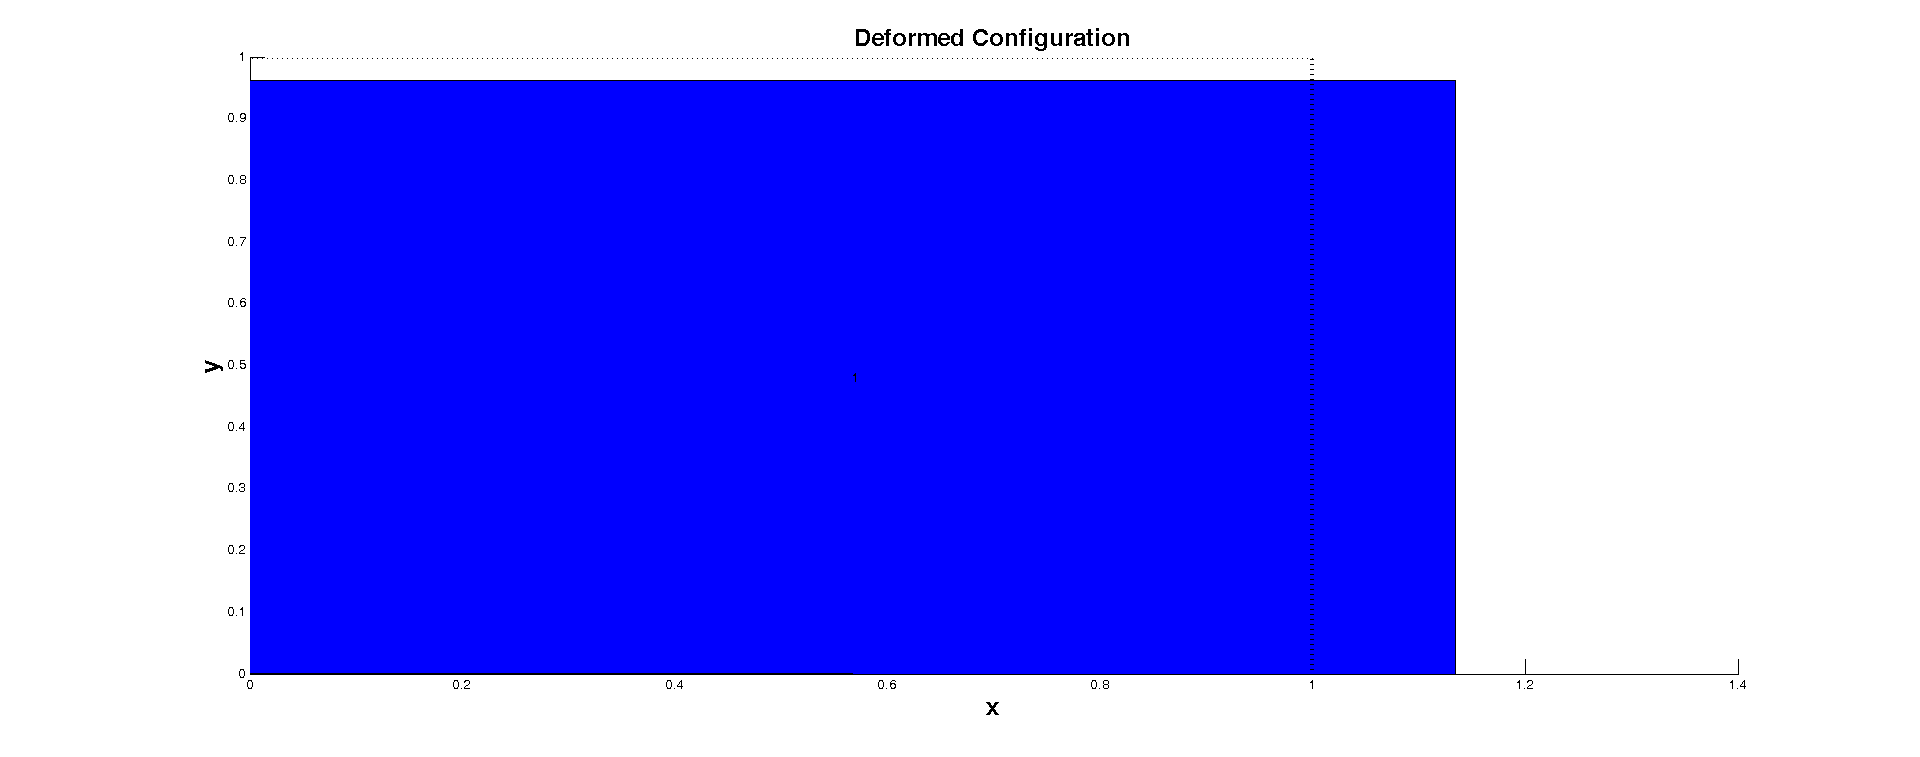
\includegraphics[width=7.0in]{Deformed3a}
\end{center}
\newpage \item Contour: 
\begin{center}
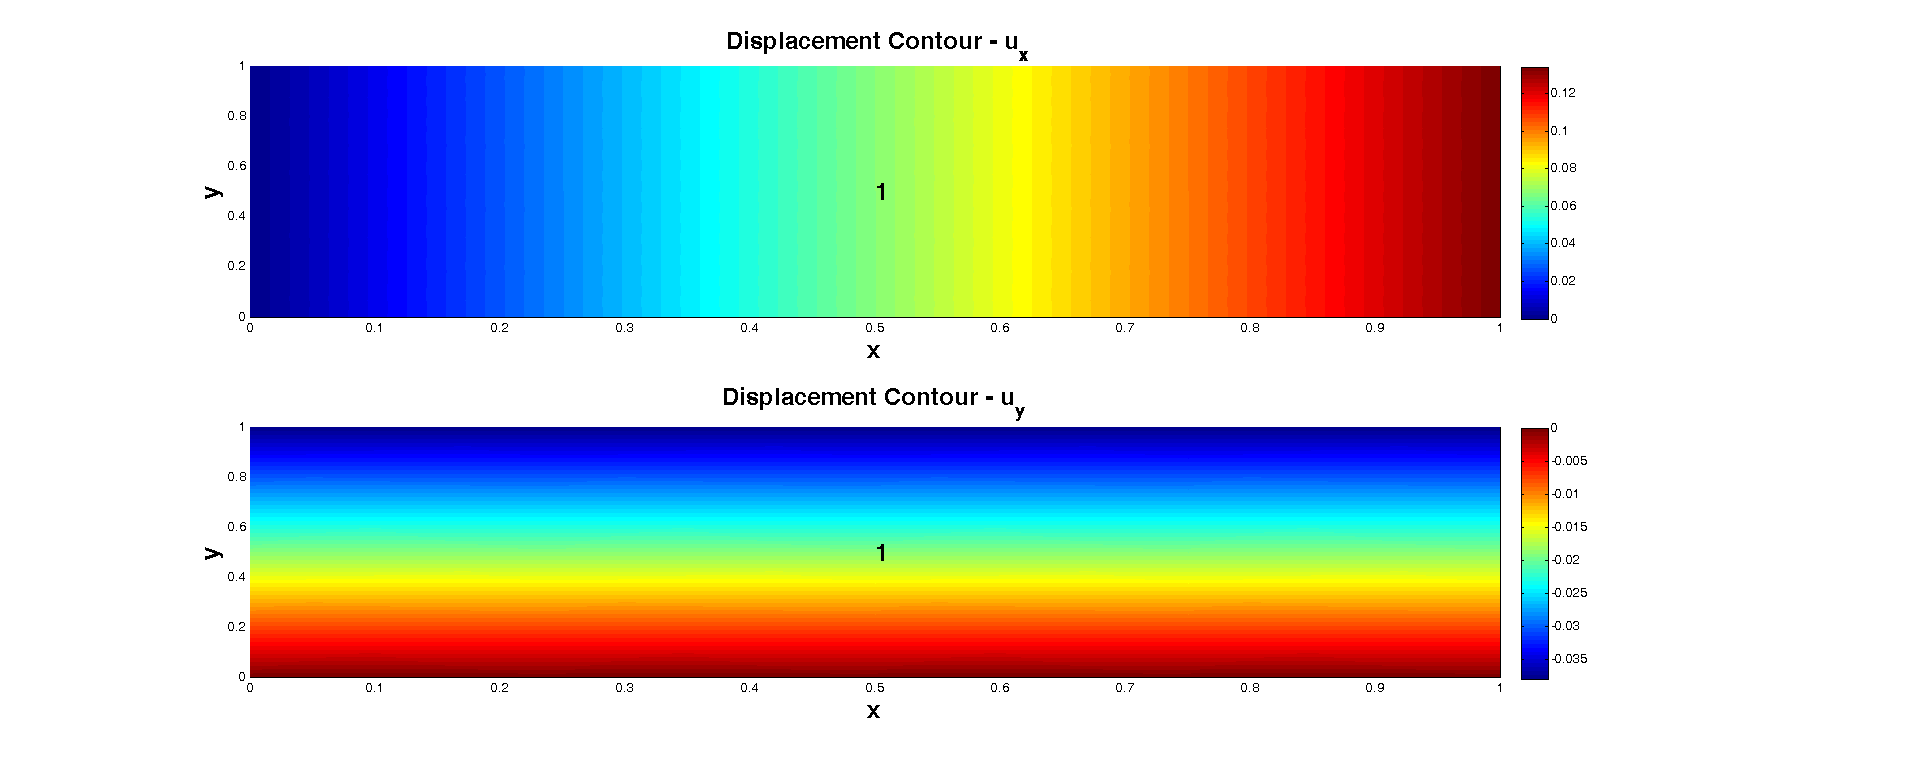
\includegraphics[width=7.0in]{Contour3a}
\end{center}
\item Stress-Strain Plot
\begin{center}
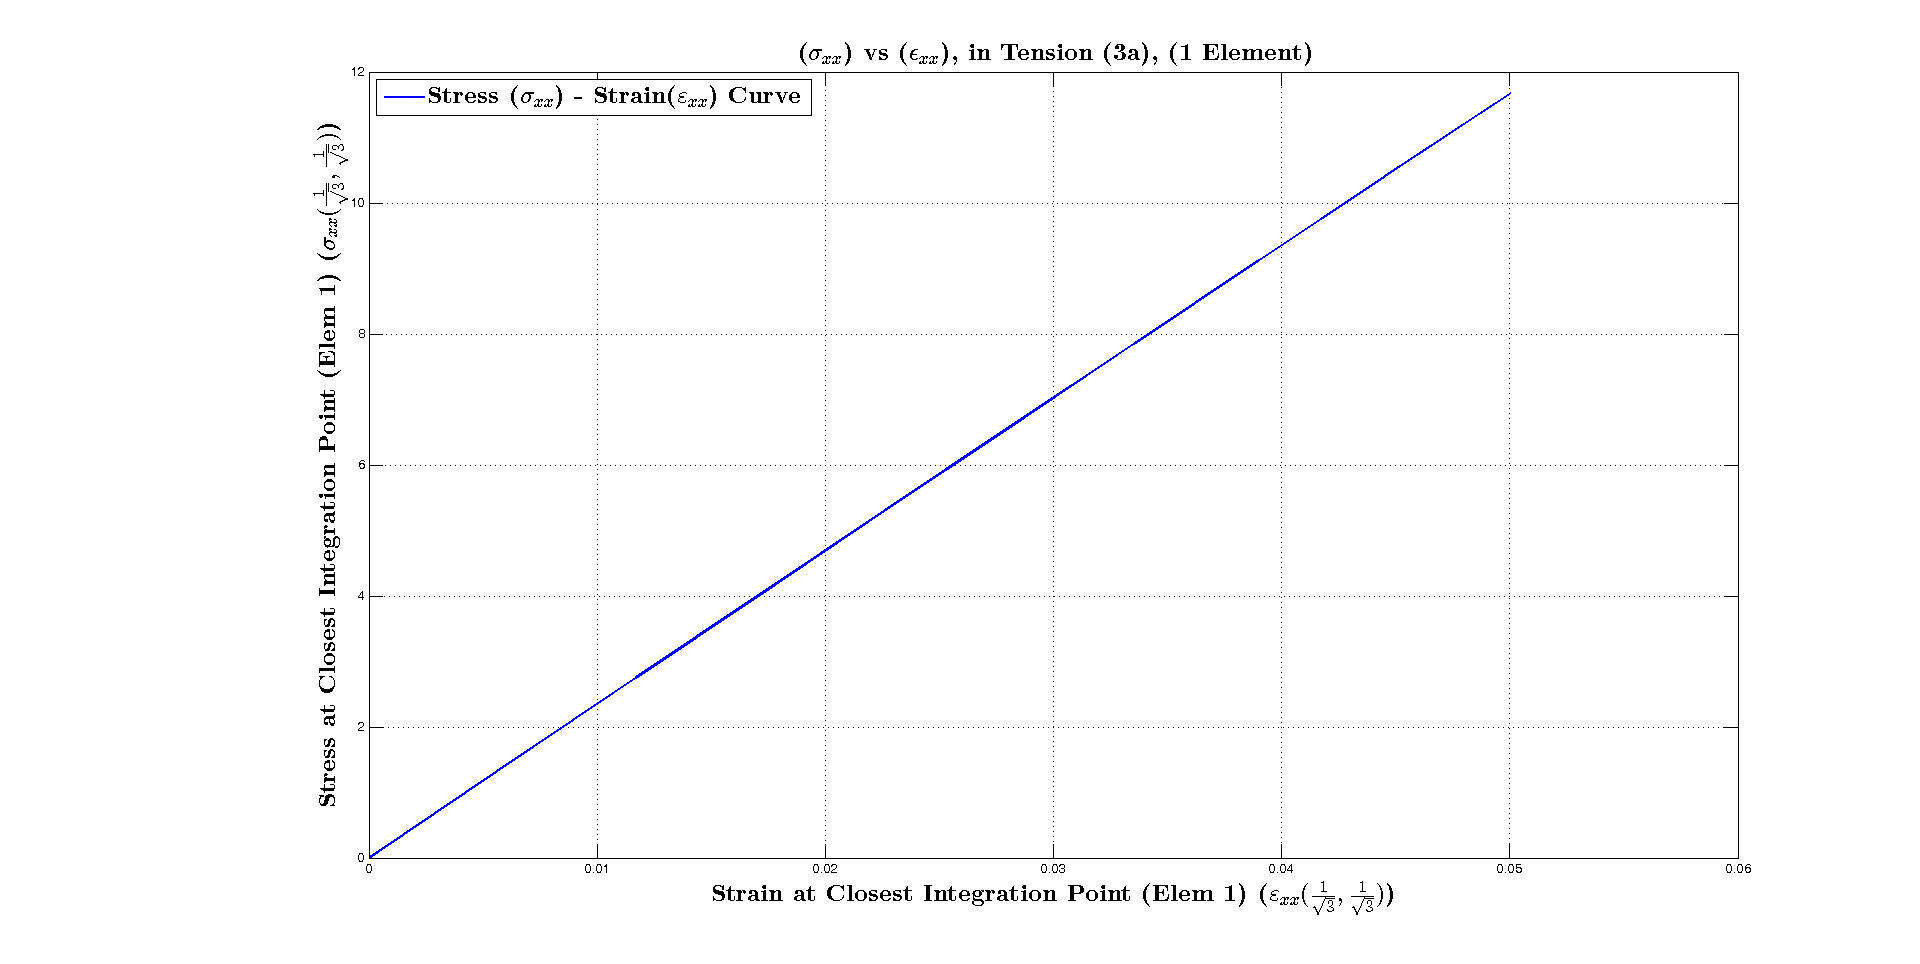
\includegraphics[width=7.0in]{Stress_Strain3a}
\end{center}
\end{itemize}
\newpage \subsection*{(b): Axial Compression}
The nodal displacements are as follows
\begin{table}[htbp]
  \centering
  \caption{Nodal Displacements for 1x1 mesh (Compression)}
    \begin{tabular}{ccc}
    \toprule
    {Node No} & {$\Delta_x$} & {$\Delta_y$} \\
    \midrule
    1     & 0     & 0 \\
    2     & -0.05003 & 0 \\
    3     & 0     & 0.01596 \\
    4     & -0.05003 & 0.01596 \\
    \bottomrule
    \end{tabular}%
  \label{Displacementscomp}%
\end{table}%
\begin{itemize}
\item Deformed Shape:
\begin{center}
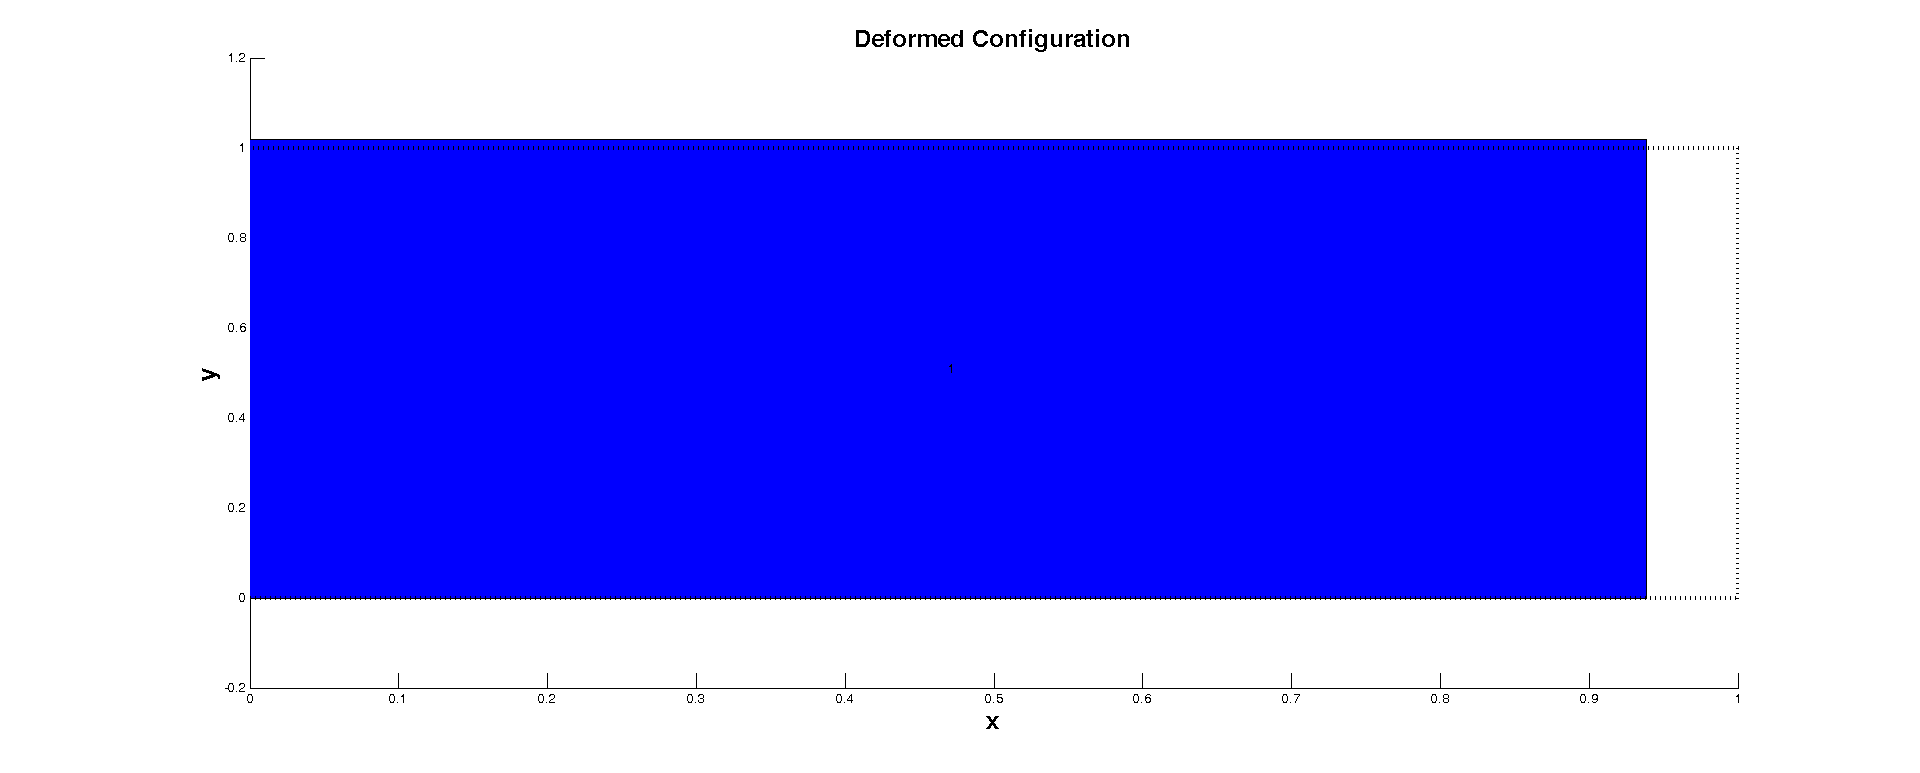
\includegraphics[width=7.0in]{Deformed3b}
\end{center} 
\newpage \item Contour: 
\begin{center}
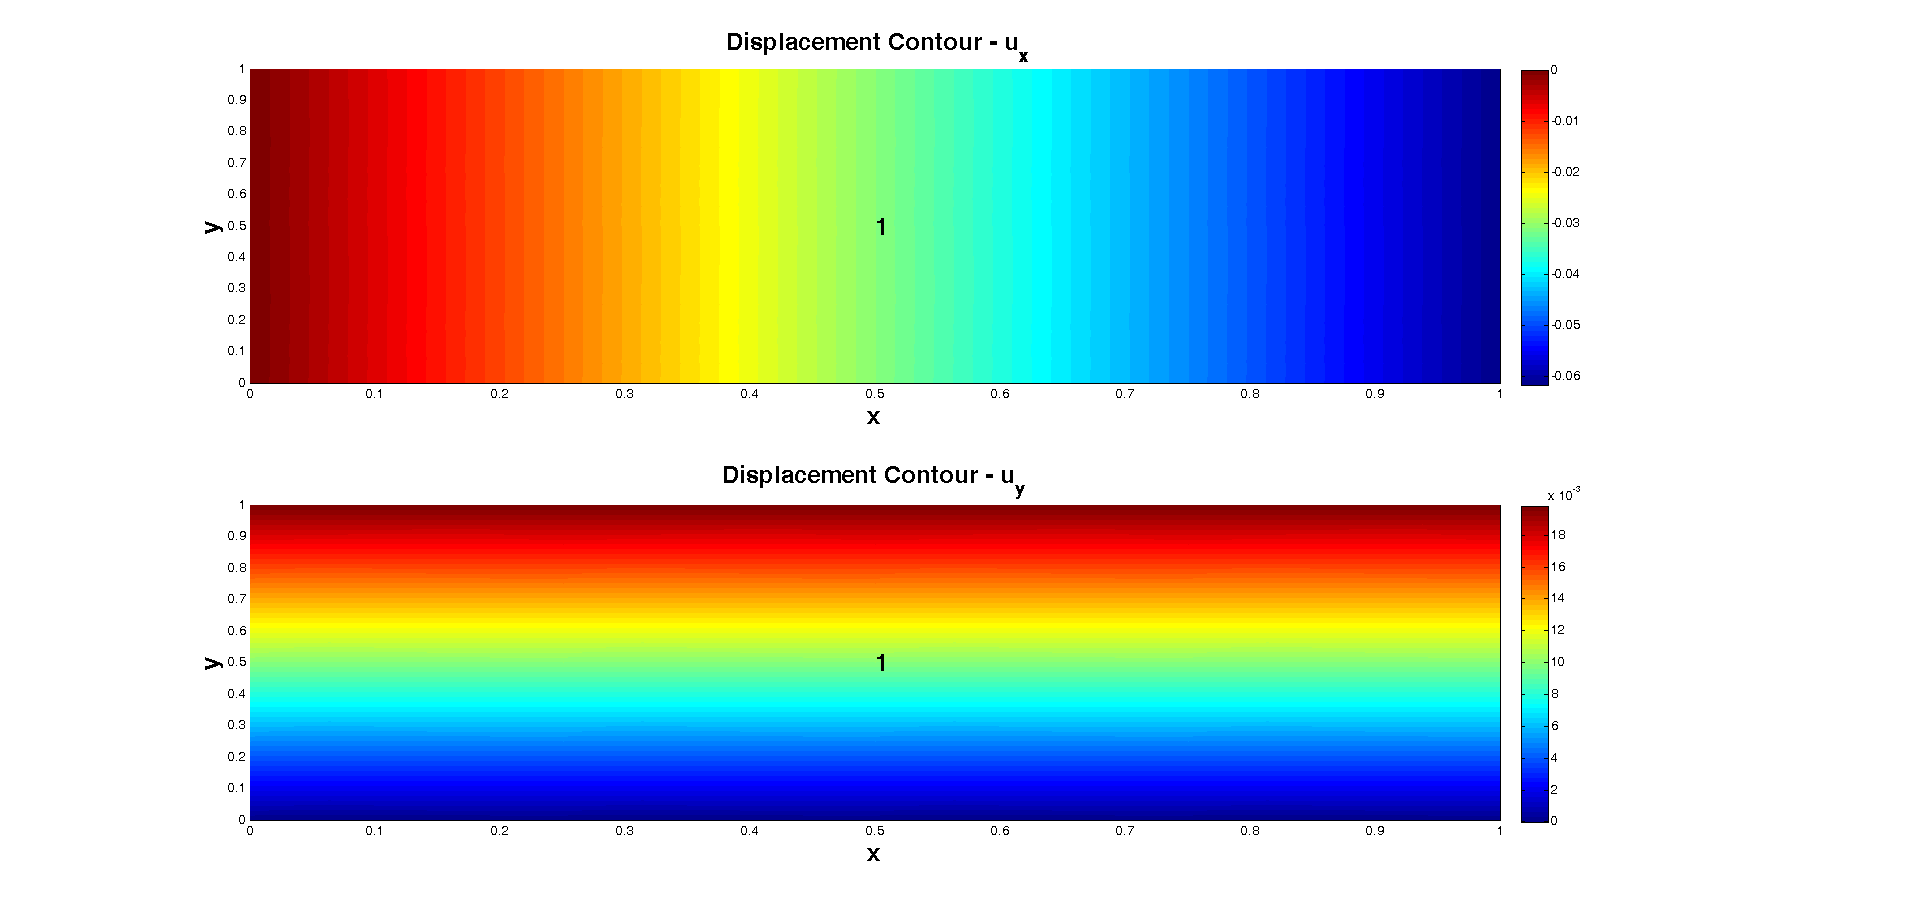
\includegraphics[width=7.0in]{Contour3b}
\end{center}
\item Stress-Strain Plot
\begin{center}
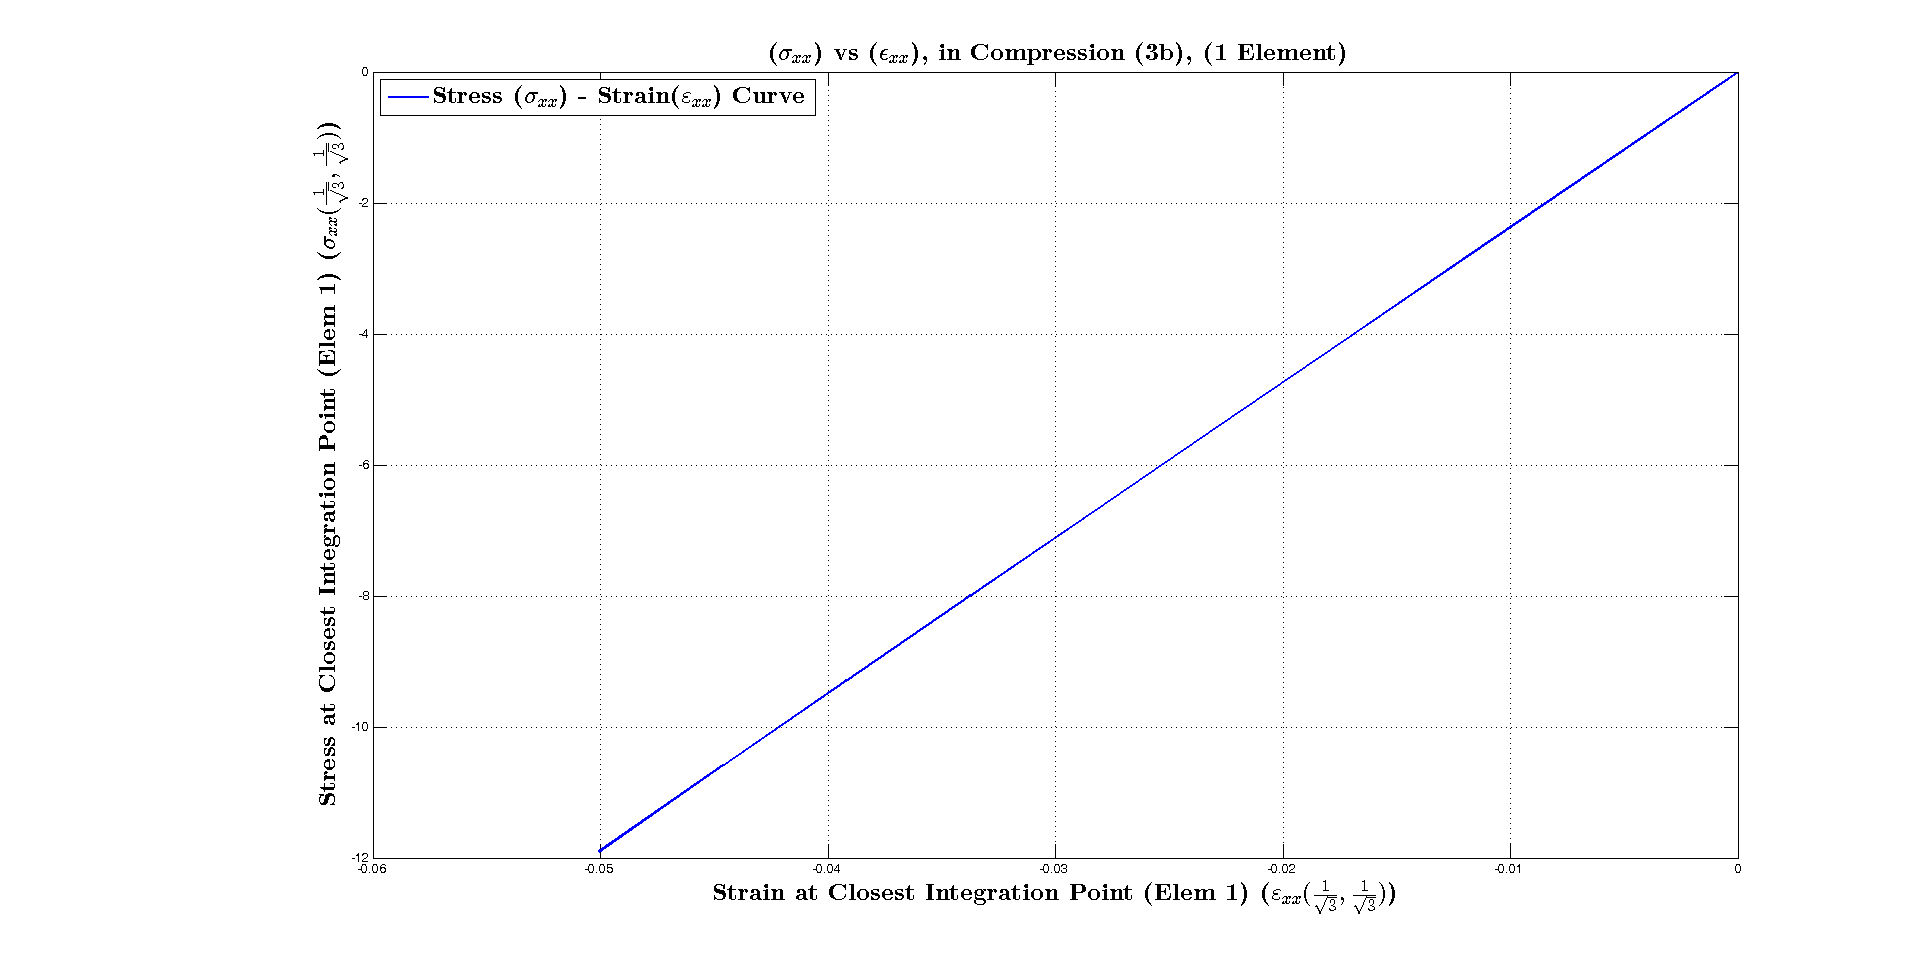
\includegraphics[width=7.0in]{Stress_Strain3b}
\end{center}
\end{itemize}
\newpage \section*{Sol$^n$ 4}
The given mesh is refined four fold in each direction.
\begin{center}
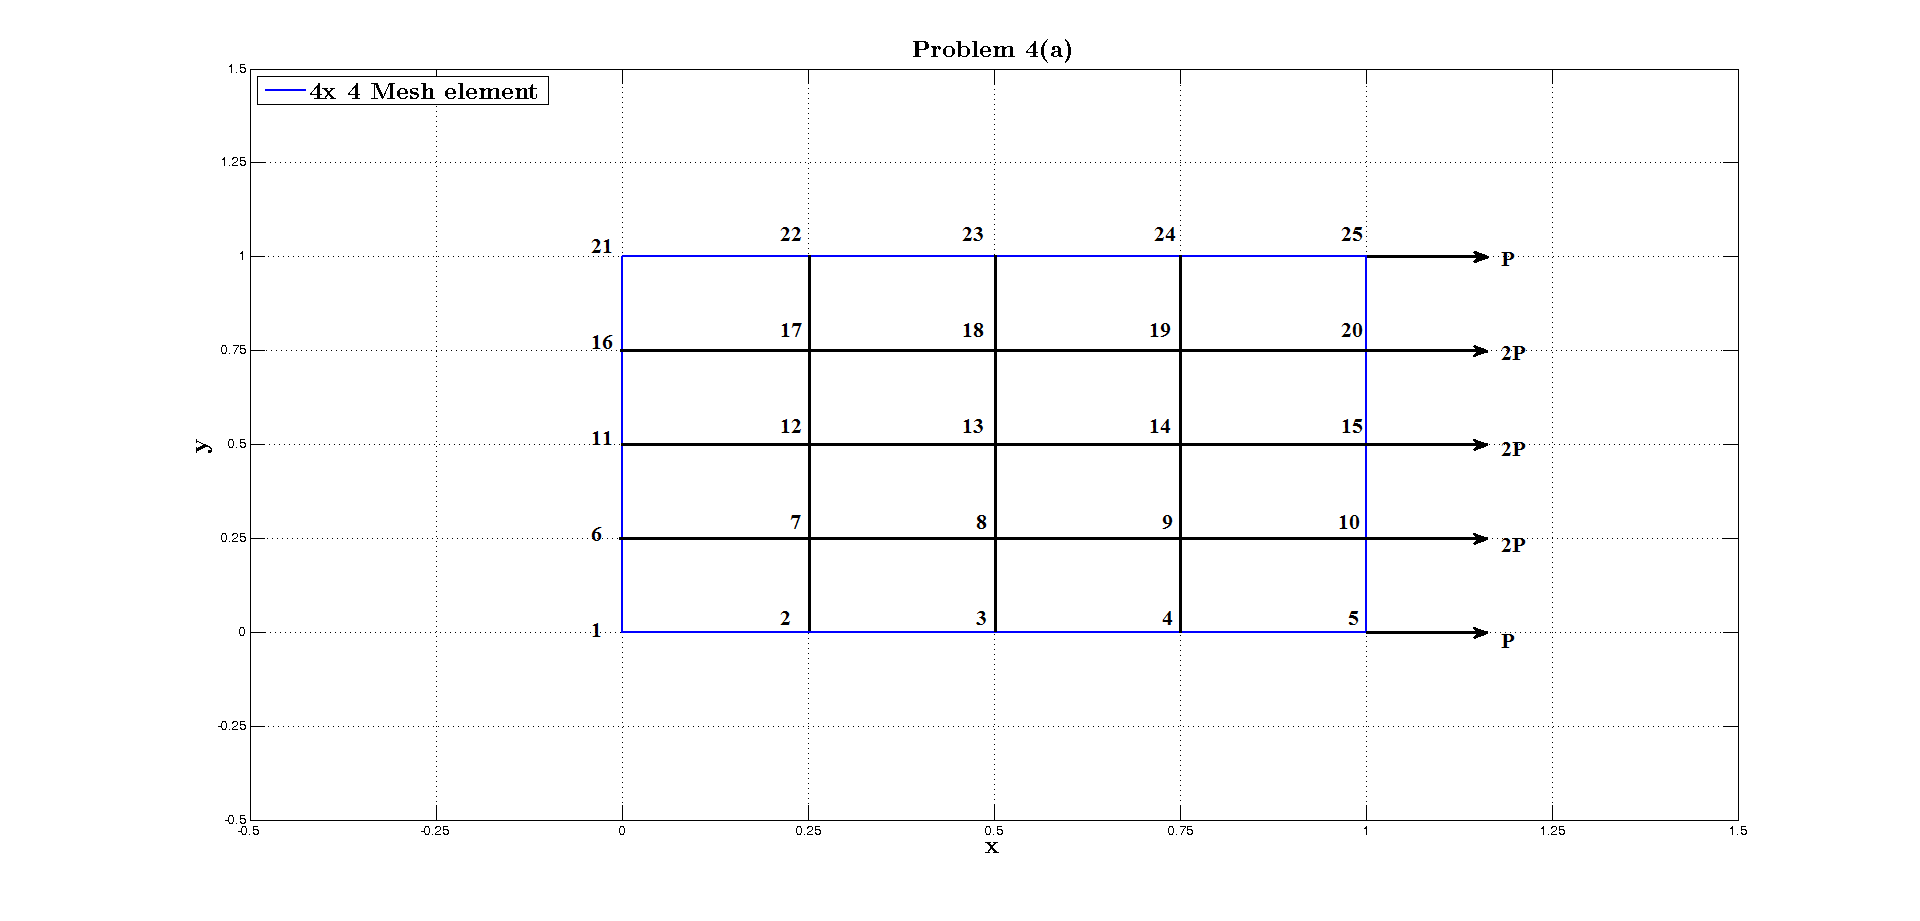
\includegraphics[width=7.5in]{fig4ael}
\end{center}
\subsection*{Comments:}
\begin{itemize}
\item The mesh refinement results in convergence, as can be seen from the displacement values obtained below. 
\item This implies that in the limit of h-refinement, we are expected to recover the exact solution. 
\item It can be seen from 3(a) that the behavior in uniaxial tension is close to linear, and hence any further refinements in the mesh would not result in any appreciable change in the stress-strain curve. 
\item It can also be noted that since the $\bf D$-matrix is dependent on strain(more precisely the trace of the strain), the behavior is expected to be different in tension and compression. This can be observed from the small difference in the peak-force values at 0.05 strain. 
\item Since we are in the small deformation regime, the trace of the strain tensor (which basically relates to the volumetric changes) doesn't undergo appreciable change throughout the course of the loading, and hence the $\bf D$-matrix itself doesn't undergo any appreciable change. Thus the obtained behavior, as from the plot, is at least, qualitatively justified.  
\begin{align*}
D_{11}
=
a\kappa + 3b\ ; \ \ \ \kappa = \frac{2+{\rm tr}{\bm\varepsilon}}{(1+{\rm tr}{\bm\varepsilon})^2}\ \ ; \ \ \ |{\rm tr}{\bm\varepsilon}|<0.05\ \ ; \ \ \kappa\approx 2
\end{align*}
\item Since the corresponding entry in the $\bf D$-matrix does not undergo any appreciable change, the number of iterations obtained for each load step are also small. And consequently using modified newton raphson would prove to be both efficient and cost saving for the given problem. This is because the $\bf D$-matrix update on each iteration is saved.
\item Since the behavior is close to linear, the changes in tolerance parameter for residual check would not make any appreciable change in the number of iterations taken to converge. And a sufficiently small tolerance (in the range of $\approx 10^{-5} - 10^{-8}$) should serve the purpose effectively. 
\end{itemize}
\subsection*{(a): }
The nodal displacements are as obtained below
\begin{table}[h!]
  \centering
  \caption{Nodal Displacements for 4x4 mesh (Tension)}
    \begin{tabular}{ccc}
    \toprule
    {Node No} & {$\Delta_x$} & {$\Delta_y$} \\
    \midrule
    1     & 0     & 0 \\
    2     & 0.01251 & 5.26E-20 \\
    3     & 0.025019 & 1.87E-18 \\
    4     & 0.037529 & 2.37E-18 \\
    5     & 0.050038 & 3.07E-18 \\
    6     & 0     & -0.00371 \\
    7     & 0.01251 & -0.00371 \\
    8     & 0.025019 & -0.00371 \\
    9     & 0.037529 & -0.00371 \\
    10    & 0.050038 & -0.00371 \\
    11    & 0     & -0.00743 \\
    12    & 0.01251 & -0.00743 \\
    13    & 0.025019 & -0.00743 \\
    14    & 0.037529 & -0.00743 \\
    15    & 0.050038 & -0.00743 \\
    16    & 0     & -0.01114 \\
    17    & 0.01251 & -0.01114 \\
    18    & 0.025019 & -0.01114 \\
    19    & 0.037529 & -0.01114 \\
    20    & 0.050038 & -0.01114 \\
    21    & 0     & -0.01485 \\
    22    & 0.01251 & -0.01485 \\
    23    & 0.025019 & -0.01485 \\
    24    & 0.037529 & -0.01485 \\
    25    & 0.050038 & -0.01485 \\
    \bottomrule
    \end{tabular}%
  \label{Displacements4a}%
\end{table}%
\newpage The contours and deformed shapes are as given below
\begin{itemize}
\item Deformed Shape:
\begin{center}
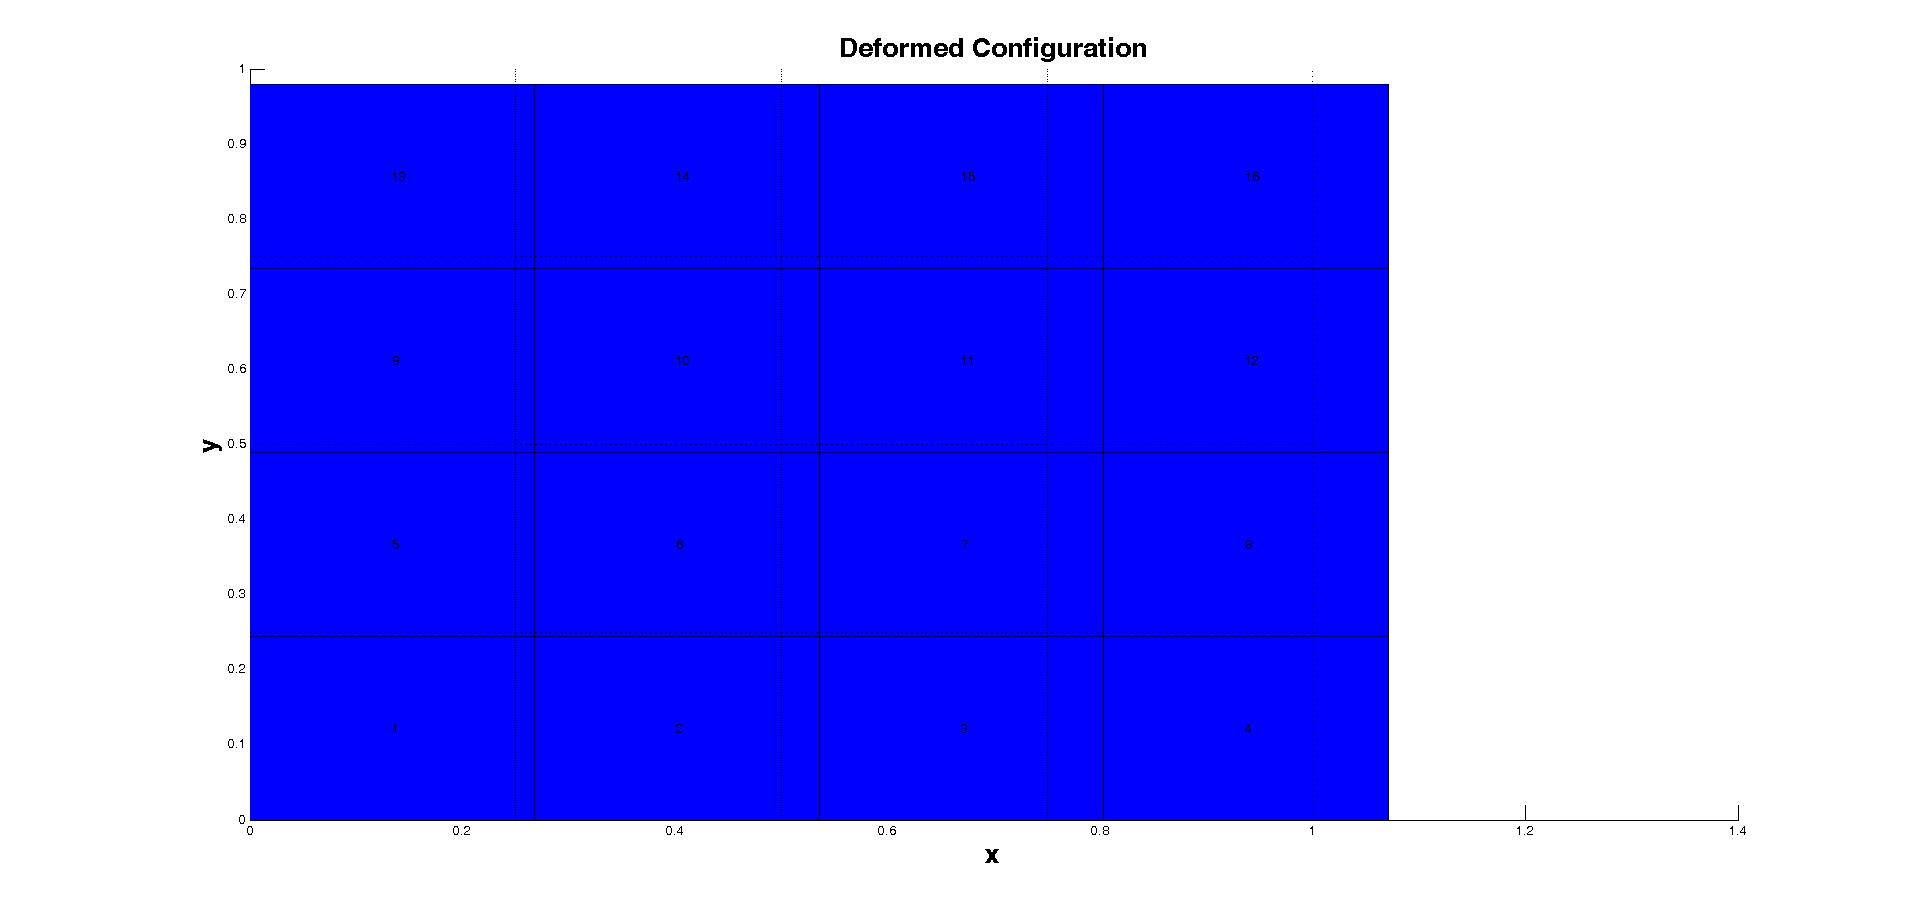
\includegraphics[width=7.0in]{Deformed4a}
\end{center}
\begin{center}
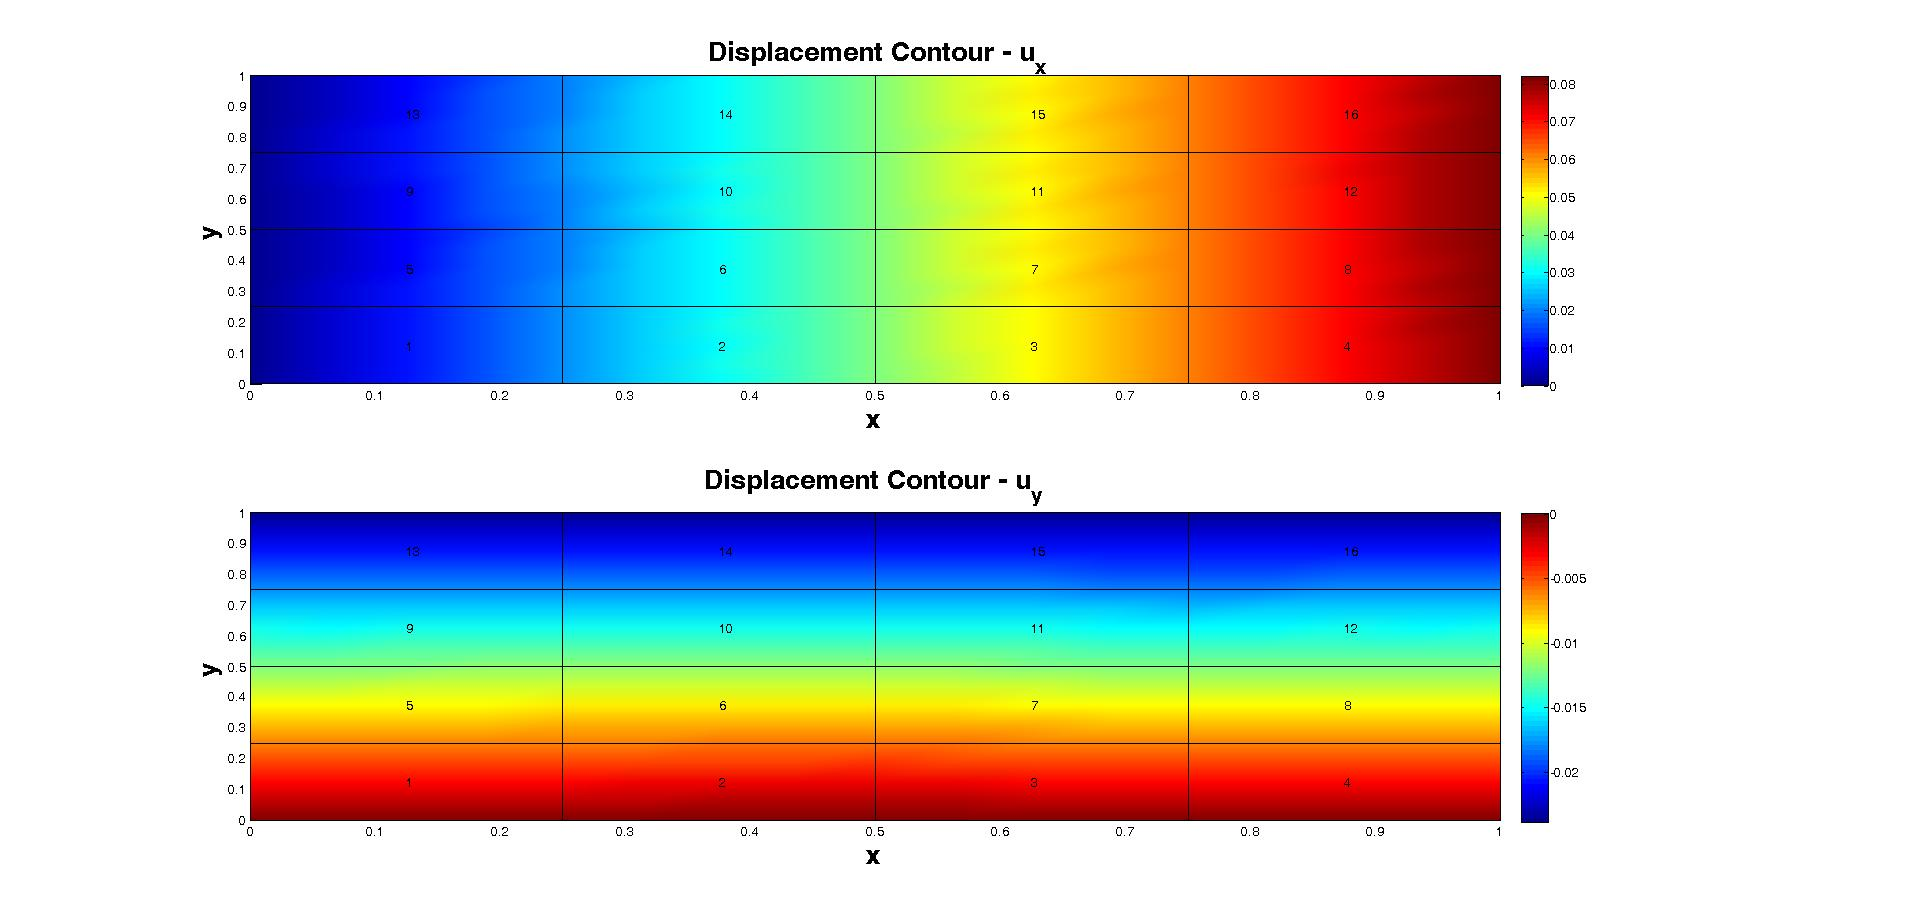
\includegraphics[width=7.0in]{Contour4a}
\end{center}
\end{itemize}
\newpage The corresponding stress strain curve for the integration point closest to the top right end of the mesh, is presented below. 
\begin{center}
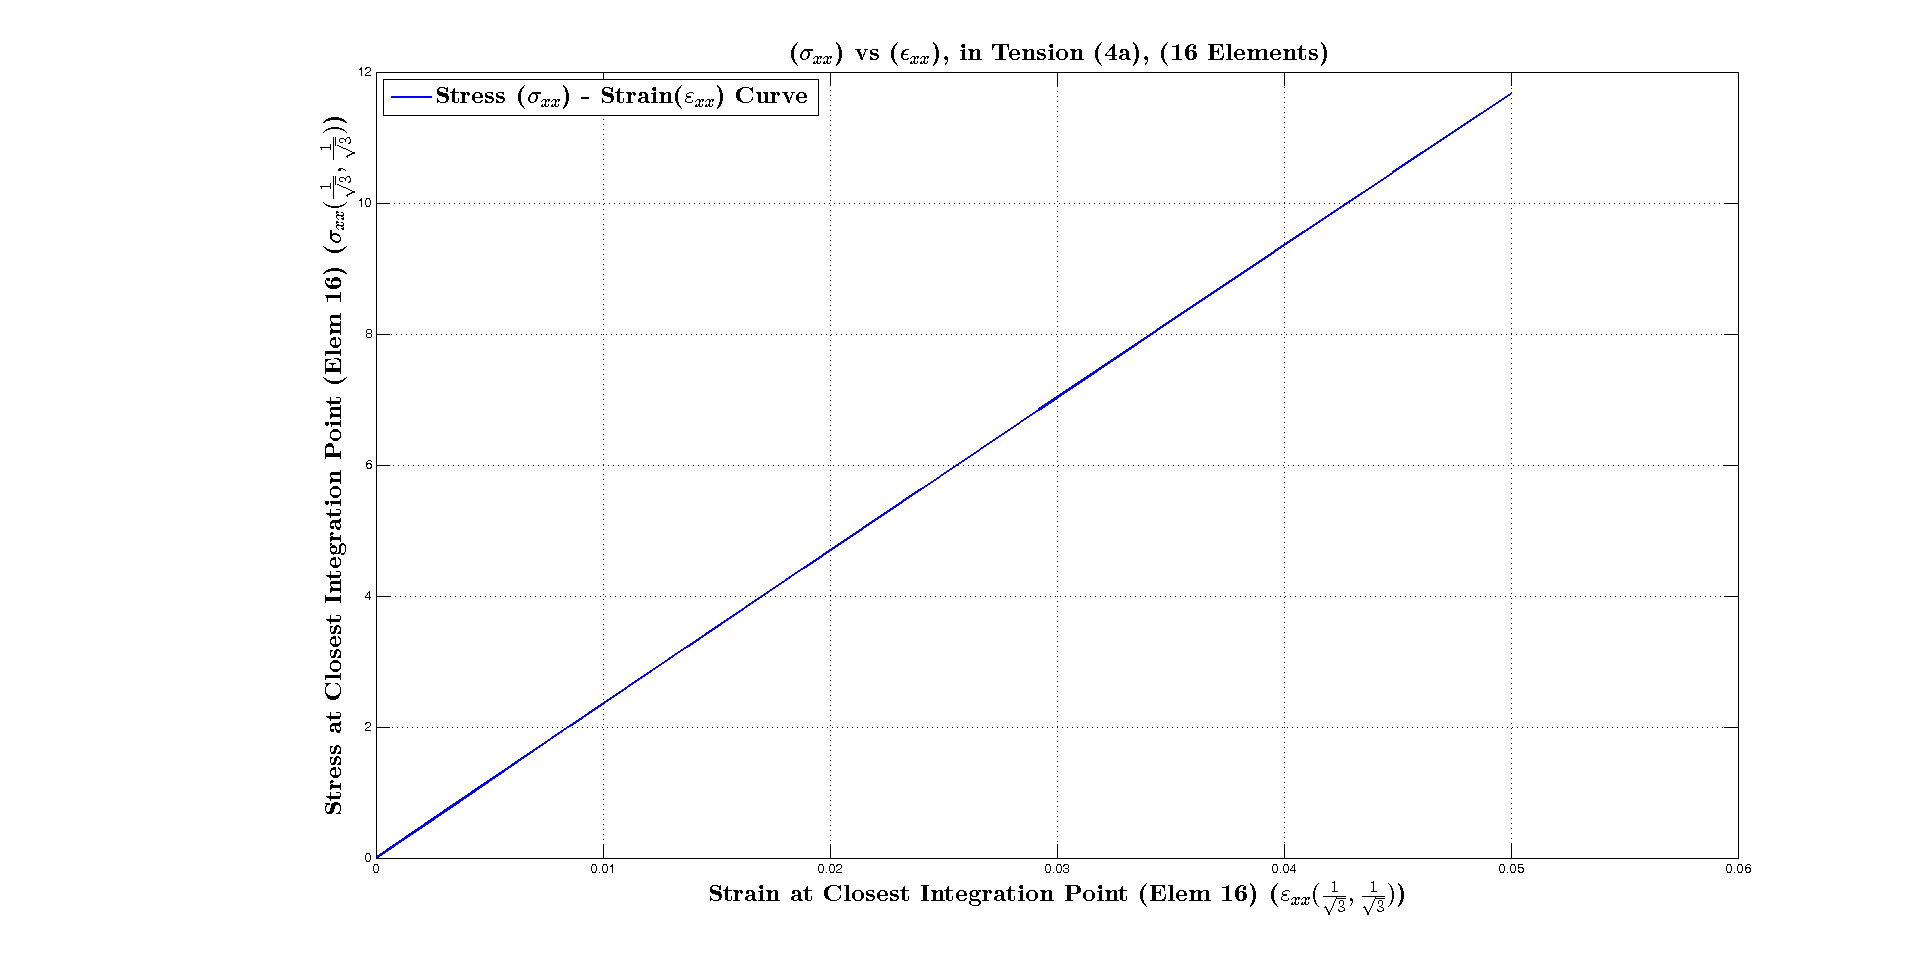
\includegraphics[width=7.0in]{Stress_Strain4a}
\end{center}
\subsection*{(b)}
For the present case, we apply shear on the right edge of the mesh. Note that the total shear force applied on the right edge is equal to 10 units. Therefore following the same principle as in 4(a), the force is equivalently divided into nodal forces such that the force at an internal node is twice the force at the extreme end.
\begin{itemize}
\item Deformed Shape
\begin{center}
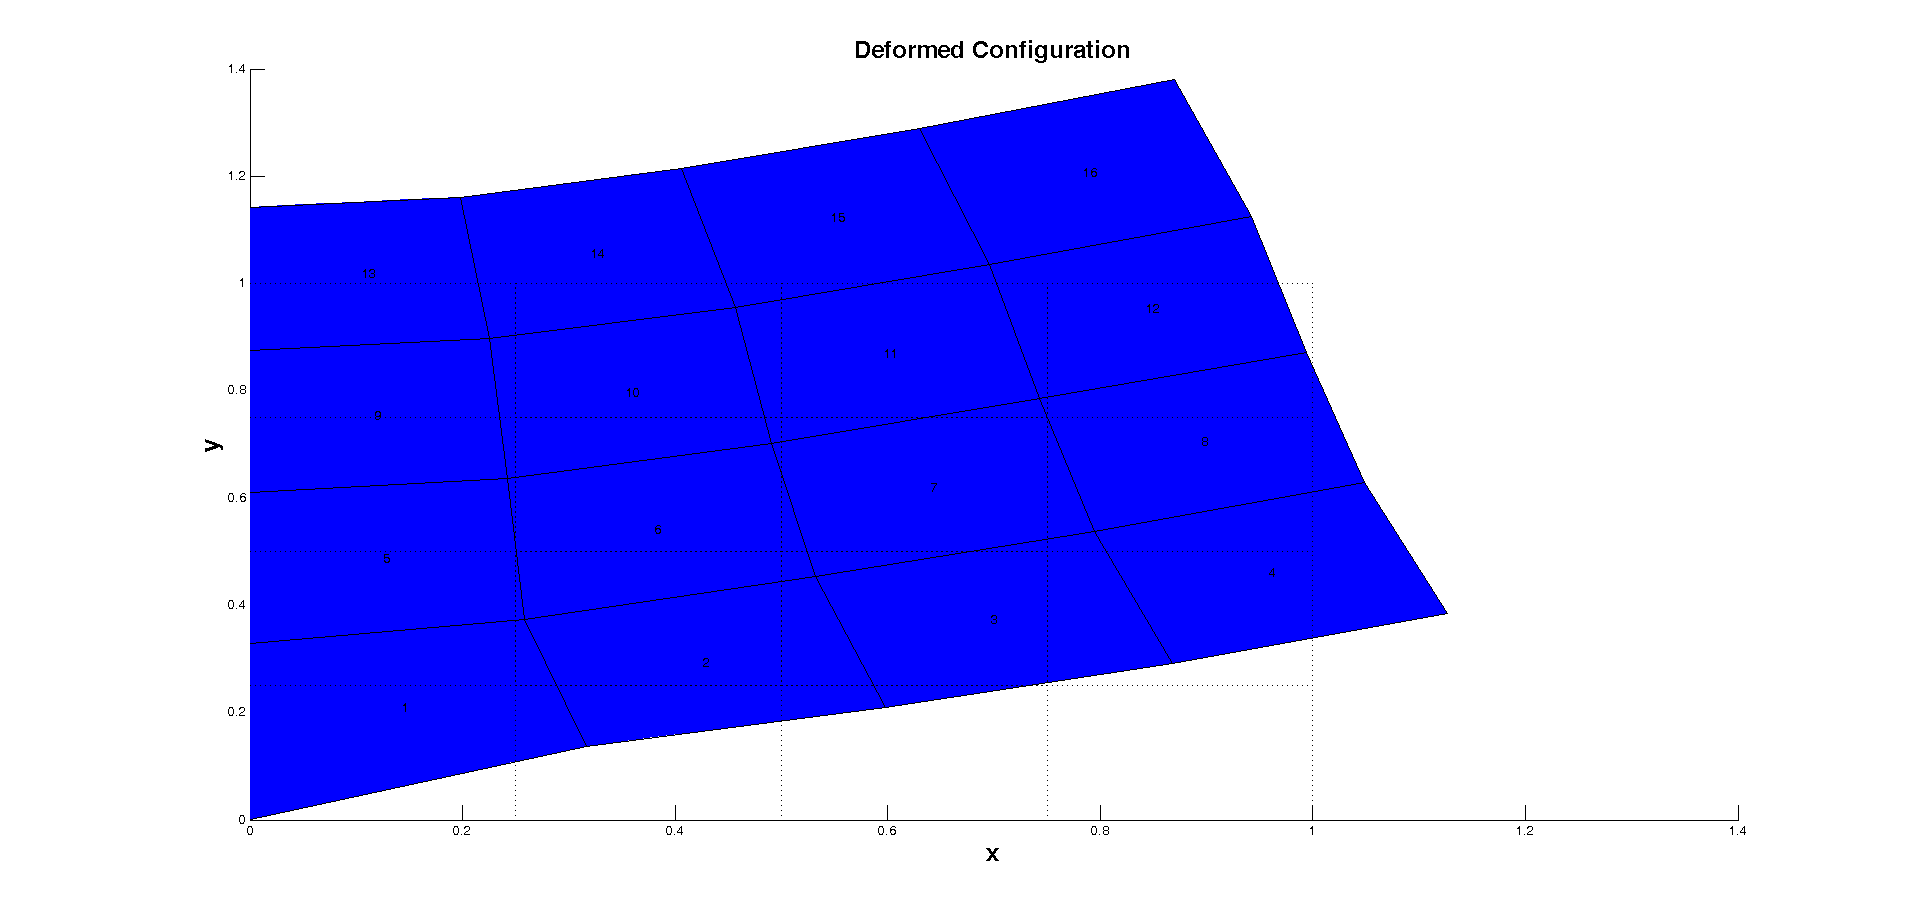
\includegraphics[width=7.0in]{Deformed4b}
\end{center}
\newpage \item Contour
\begin{center}
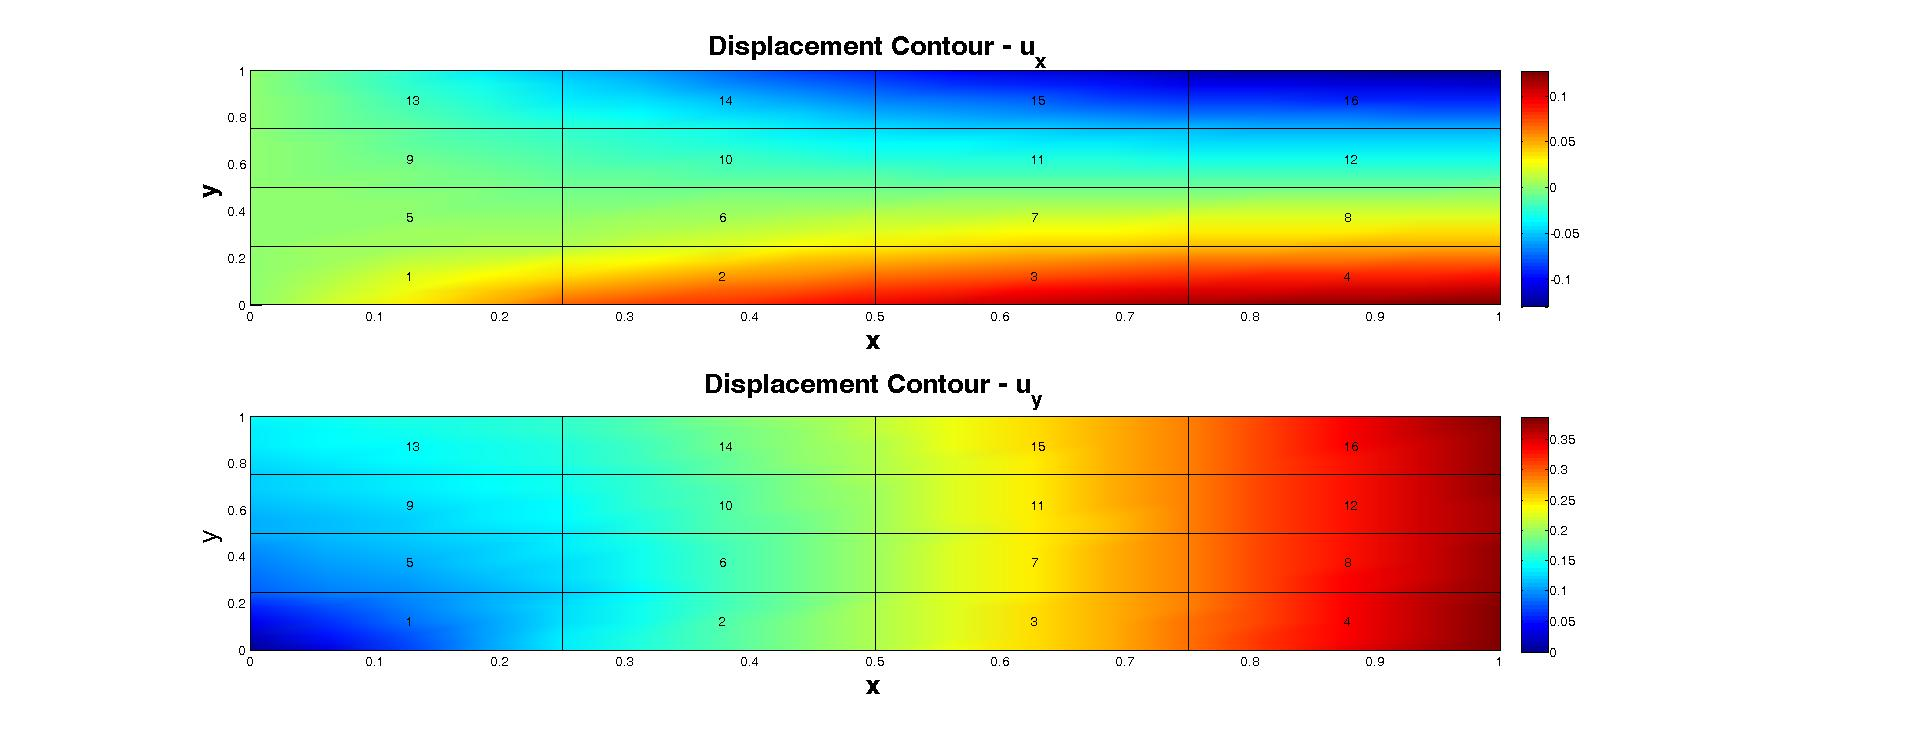
\includegraphics[width=7.0in]{Contour4b}
\end{center}
\end{itemize} 
The corresponding stress-strain plot is given below
\begin{center}
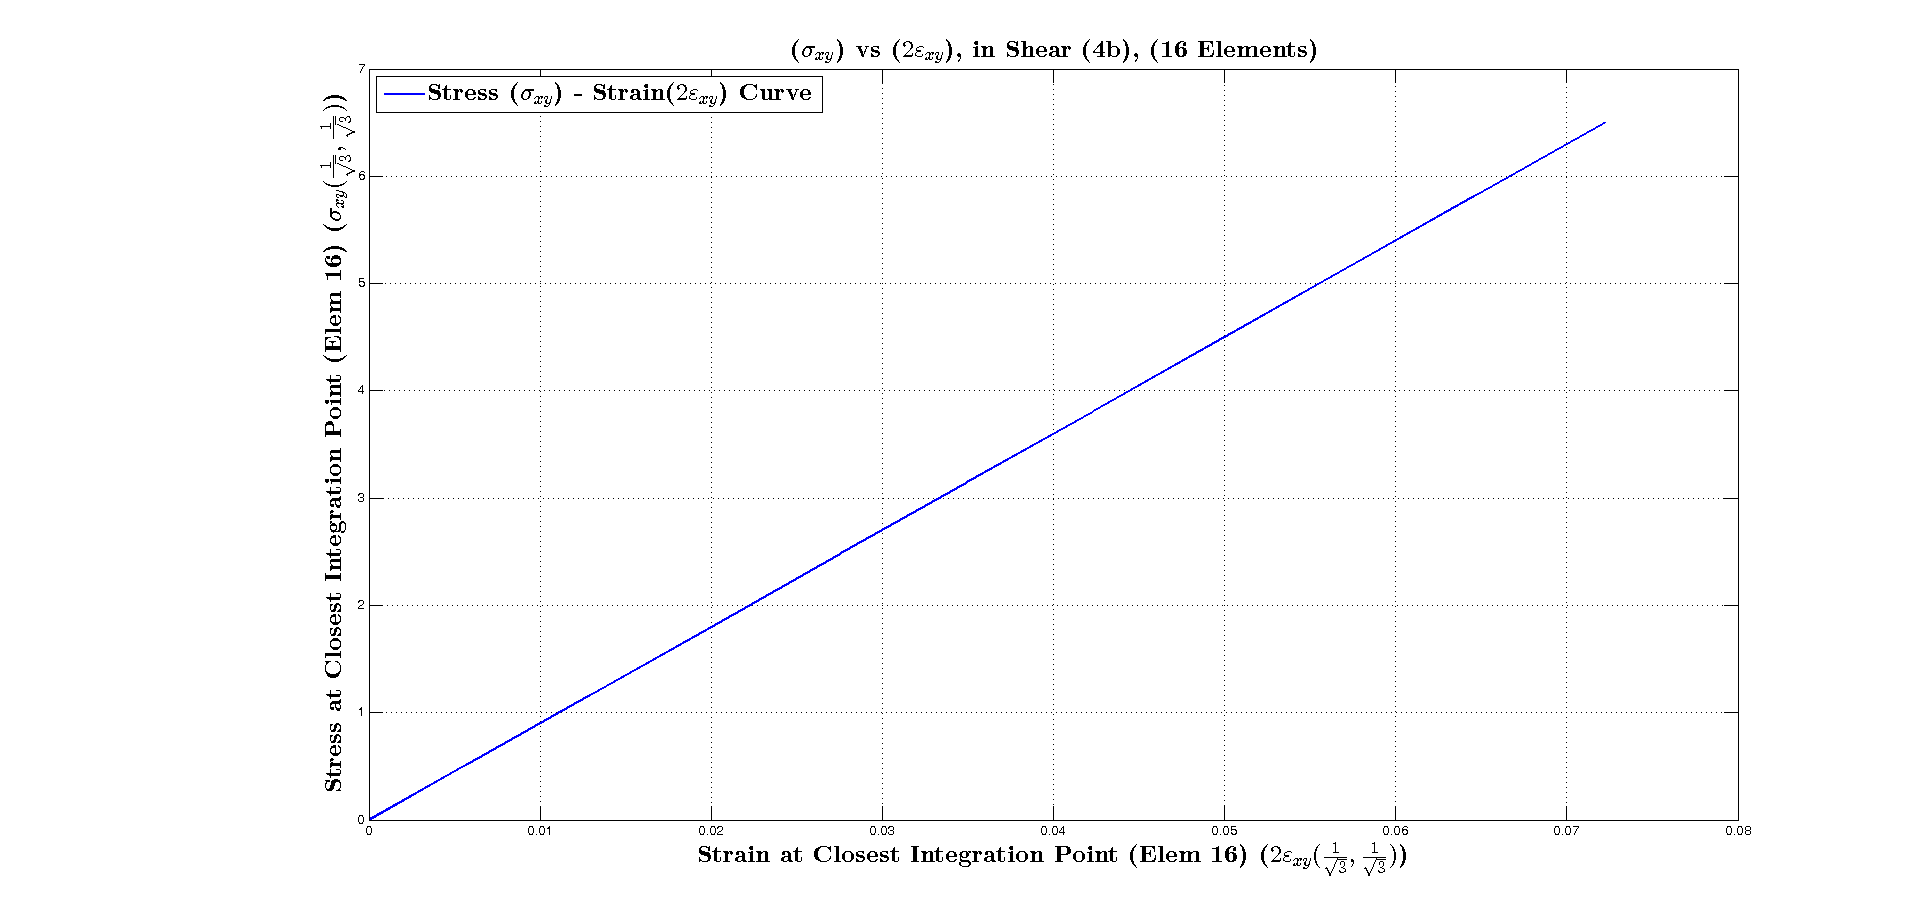
\includegraphics[width=7.5in]{Stress_Strain4b}
\end{center}
\newpage Additionally, if $\varepsilon_{xy}$ is used instead of $2\varepsilon_{xy}$ on the x-axis, the following plot is obtained. 
\begin{center}
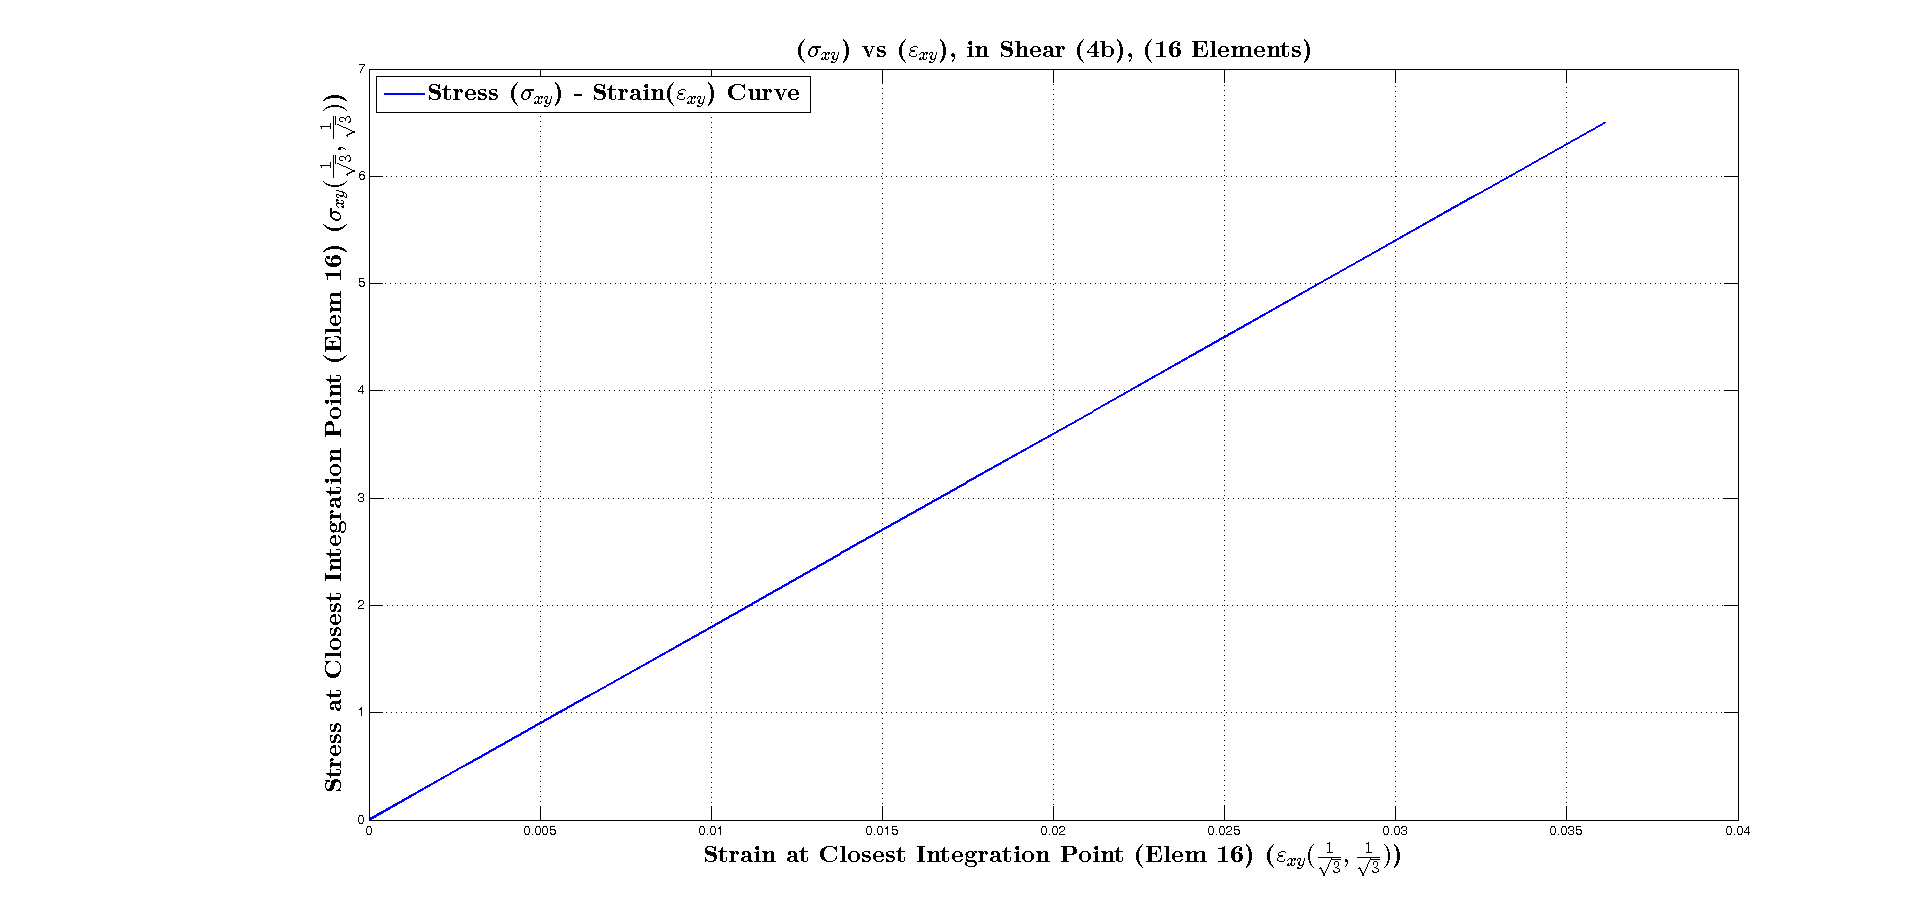
\includegraphics[width=7.5in]{Stress_Strain4bh}
\end{center}
 The nodal displacements are given on the next page
\begin{table}[h!]
  \centering
  \caption{Nodal Displacements for 4x4 mesh (Shear)}
    \begin{tabular}{ccc}
    \toprule
    Node No & $\Delta_x$    & $\Delta_y$ \\
    \midrule
    1     & 0     & 0 \\
    2     & 0.066795 & 0.136885 \\
    3     & 0.097843 & 0.209438 \\
    4     & 0.11793 & 0.290916 \\
    5     & 0.126508 & 0.385225 \\
    6     & 0     & 0.07909 \\
    7     & 0.008424 & 0.124064 \\
    8     & 0.032302 & 0.204317 \\
    9     & 0.044306 & 0.287492 \\
    10    & 0.048853 & 0.378639 \\
    11    & 0     & 0.109904 \\
    12    & -0.00743 & 0.135831 \\
    13    & -0.00929 & 0.201331 \\
    14    & -0.00707 & 0.28569 \\
    15    & -0.00591 & 0.371586 \\
    16    & 0     & 0.126016 \\
    17    & -0.02455 & 0.147421 \\
    18    & -0.04349 & 0.205089 \\
    19    & -0.05403 & 0.285297 \\
    20    & -0.05767 & 0.37432 \\
    21    & 0     & 0.141956 \\
    22    & -0.05165 & 0.161125 \\
    23    & -0.09356 & 0.213804 \\
    24    & -0.12024 & 0.288636 \\
    25    & -0.1304 & 0.379496 \\
    \bottomrule
    \end{tabular}%
  \label{Displacements4b}%
\end{table}%
\subsection*{Comments}
The following comments are worth noting the context of shear deformation. 
\begin{itemize}
\item The stress-strain curve, unlike the case of compression or tension, is exactly linear. 
\item This is due to the fact that the corresponding entry in the stiffness matrix $({\bf D(\bm\varepsilon)}[3,3])$, is constant and equal to $3b/2$ . \\ \hrule 
\end{itemize}
\section*{Appendix: Stress-Strain Tables for 4(a) and 4(b)}
\begin{itemize}
\item The stress-strain tables obtained for various loading cases are attached below, for reference. 
\item The entries in these correspond to the stress (and strain) values at the integration point closest to the top right corner of the mesh, obtained at each iteration during the loading. 
\item Since force, type boundary condition is prescribed, the iterations are performed until the strain value at the integration point just crosses the prescribed limit ($|\varepsilon_{xx}\left(\frac{1}{\sqrt{3}},\frac{1}{\sqrt{3}}\right)| \leq 0.05$). Here the coordinates describe the location of the integration point in the canonical ($\xi-\eta$) domain
\item For the case of the shear loading, the load is applied without any restriction on the maximum strain value at the integration point. 
\end{itemize}
\newpage \subsection*{Instructions for Running the code:}
The following instructions are relevant for running the code.  
\begin{itemize}
\item For 3(a) , in tension, for 1x1 mesh switch the following parameters: as instructed in the code
\begin{itemize}
\item Comment in the input file , (Line 117-124), uncomment line 126.
\item Comment line 176.
\item Uncomment line 177-178
\item Uncomment line 110-113
\item Comment line 94
\end{itemize}
\item For 3(b) Multiply the Node\_Loads with a $'-1'$. (Line 177-178)
\item For 4(a) The procedure is exactly the reverse of the above. 
\begin{itemize}
\item Unomment in the input file , (Line 117-124), uncomment line 126.
\item Uncomment line 176.
\item Comment line 177-178
\item Comment line 110-113 and Unomment line 94
\end{itemize}
\item For 4(b) Introduce a 2 in front of line 179. In short, comment 177-178 and uncomment line 179-180 
\end{itemize}
\end{document}